\documentclass[twoside]{book}

% Packages required by doxygen
\usepackage{fixltx2e}
\usepackage{calc}
\usepackage{doxygen}
\usepackage[export]{adjustbox} % also loads graphicx
\usepackage{graphicx}
\usepackage[utf8]{inputenc}
\usepackage{makeidx}
\usepackage{multicol}
\usepackage{multirow}
\PassOptionsToPackage{warn}{textcomp}
\usepackage{textcomp}
\usepackage[nointegrals]{wasysym}
\usepackage[table]{xcolor}

% NLS support packages
\usepackage[french]{babel}

% Font selection
\usepackage[T1]{fontenc}
\usepackage[scaled=.90]{helvet}
\usepackage{courier}
\usepackage{amssymb}
\usepackage{sectsty}
\renewcommand{\familydefault}{\sfdefault}
\allsectionsfont{%
  \fontseries{bc}\selectfont%
  \color{darkgray}%
}
\renewcommand{\DoxyLabelFont}{%
  \fontseries{bc}\selectfont%
  \color{darkgray}%
}
\newcommand{\+}{\discretionary{\mbox{\scriptsize$\hookleftarrow$}}{}{}}

% Page & text layout
\usepackage{geometry}
\geometry{%
  a4paper,%
  top=2.5cm,%
  bottom=2.5cm,%
  left=2.5cm,%
  right=2.5cm%
}
\tolerance=750
\hfuzz=15pt
\hbadness=750
\setlength{\emergencystretch}{15pt}
\setlength{\parindent}{0cm}
\setlength{\parskip}{3ex plus 2ex minus 2ex}
\makeatletter
\renewcommand{\paragraph}{%
  \@startsection{paragraph}{4}{0ex}{-1.0ex}{1.0ex}{%
    \normalfont\normalsize\bfseries\SS@parafont%
  }%
}
\renewcommand{\subparagraph}{%
  \@startsection{subparagraph}{5}{0ex}{-1.0ex}{1.0ex}{%
    \normalfont\normalsize\bfseries\SS@subparafont%
  }%
}
\makeatother

% Headers & footers
\usepackage{fancyhdr}
\pagestyle{fancyplain}
\fancyhead[LE]{\fancyplain{}{\bfseries\thepage}}
\fancyhead[CE]{\fancyplain{}{}}
\fancyhead[RE]{\fancyplain{}{\bfseries\leftmark}}
\fancyhead[LO]{\fancyplain{}{\bfseries\rightmark}}
\fancyhead[CO]{\fancyplain{}{}}
\fancyhead[RO]{\fancyplain{}{\bfseries\thepage}}
\fancyfoot[LE]{\fancyplain{}{}}
\fancyfoot[CE]{\fancyplain{}{}}
\fancyfoot[RE]{\fancyplain{}{\bfseries\scriptsize Généré par Doxygen }}
\fancyfoot[LO]{\fancyplain{}{\bfseries\scriptsize Généré par Doxygen }}
\fancyfoot[CO]{\fancyplain{}{}}
\fancyfoot[RO]{\fancyplain{}{}}
\renewcommand{\footrulewidth}{0.4pt}
\renewcommand{\chaptermark}[1]{%
  \markboth{#1}{}%
}
\renewcommand{\sectionmark}[1]{%
  \markright{\thesection\ #1}%
}

% Indices & bibliography
\usepackage{natbib}
\usepackage[titles]{tocloft}
\setcounter{tocdepth}{3}
\setcounter{secnumdepth}{5}
\makeindex

% Hyperlinks (required, but should be loaded last)
\usepackage{ifpdf}
\ifpdf
  \usepackage[pdftex,pagebackref=true]{hyperref}
\else
  \usepackage[ps2pdf,pagebackref=true]{hyperref}
\fi
\hypersetup{%
  colorlinks=true,%
  linkcolor=blue,%
  citecolor=blue,%
  unicode%
}

% Custom commands
\newcommand{\clearemptydoublepage}{%
  \newpage{\pagestyle{empty}\cleardoublepage}%
}

\usepackage{caption}
\captionsetup{labelsep=space,justification=centering,font={bf},singlelinecheck=off,skip=4pt,position=top}

%===== C O N T E N T S =====

\begin{document}

% Titlepage & ToC
\hypersetup{pageanchor=false,
             bookmarksnumbered=true,
             pdfencoding=unicode
            }
\pagenumbering{roman}
\begin{titlepage}
\vspace*{7cm}
\begin{center}%
{\Large Bataille Navale }\\
\vspace*{1cm}
{\large Généré par Doxygen 1.8.11}\\
\end{center}
\end{titlepage}
\clearemptydoublepage
\tableofcontents
\clearemptydoublepage
\pagenumbering{arabic}
\hypersetup{pageanchor=true}

%--- Begin generated contents ---
\chapter{Index hiérarchique}
\section{Hiérarchie des classes}
Cette liste d\textquotesingle{}héritage est classée approximativement par ordre alphabétique \+:\begin{DoxyCompactList}
\item \contentsline{section}{Grille}{\pageref{class_grille}}{}
\item \contentsline{section}{Jeu\+Bataille\+Navale}{\pageref{class_jeu_bataille_navale}}{}
\item \contentsline{section}{Joueur}{\pageref{class_joueur}}{}
\begin{DoxyCompactList}
\item \contentsline{section}{Joueur\+Humain}{\pageref{class_joueur_humain}}{}
\item \contentsline{section}{Joueur\+IA}{\pageref{class_joueur_i_a}}{}
\end{DoxyCompactList}
\end{DoxyCompactList}

\chapter{Index des classes}
\section{Liste des classes}
Liste des classes, structures, unions et interfaces avec une brève description \+:\begin{DoxyCompactList}
\item\contentsline{section}{\hyperlink{class_grille}{Grille} }{\pageref{class_grille}}{}
\item\contentsline{section}{\hyperlink{class_jeu_bataille_navale}{Jeu\+Bataille\+Navale} }{\pageref{class_jeu_bataille_navale}}{}
\item\contentsline{section}{\hyperlink{class_joueur}{Joueur} }{\pageref{class_joueur}}{}
\item\contentsline{section}{\hyperlink{class_joueur_humain}{Joueur\+Humain} \\*Classe representant le joueur qui est humain. Cette classe hérite de la classe \hyperlink{class_joueur}{Joueur} }{\pageref{class_joueur_humain}}{}
\item\contentsline{section}{\hyperlink{class_joueur_i_a}{Joueur\+IA} \\*Classe representant le joueur qui est IA. Cette classe hérite de la classe \hyperlink{class_joueur}{Joueur} }{\pageref{class_joueur_i_a}}{}
\end{DoxyCompactList}

\chapter{Index des fichiers}
\section{Liste des fichiers}
Liste de tous les fichiers documentés avec une brève description \+:\begin{DoxyCompactList}
\item\contentsline{section}{/home/lucas/\+Documents/\+Git\+Hub/\+Bataille-\/\+Navale/src/\hyperlink{_affichage_8hpp}{Affichage.\+hpp} \\*Classe \hyperlink{class_affichage}{Affichage} }{\pageref{_affichage_8hpp}}{}
\item\contentsline{section}{/home/lucas/\+Documents/\+Git\+Hub/\+Bataille-\/\+Navale/src/\hyperlink{_bateau_8hpp}{Bateau.\+hpp} \\*Classe \hyperlink{class_bateau}{Bateau} }{\pageref{_bateau_8hpp}}{}
\item\contentsline{section}{/home/lucas/\+Documents/\+Git\+Hub/\+Bataille-\/\+Navale/src/\hyperlink{_gestion_sauvegarde_8hpp}{Gestion\+Sauvegarde.\+hpp} \\*Classe \hyperlink{class_gestion_sauvegarde}{Gestion\+Sauvegarde} }{\pageref{_gestion_sauvegarde_8hpp}}{}
\item\contentsline{section}{/home/lucas/\+Documents/\+Git\+Hub/\+Bataille-\/\+Navale/src/\hyperlink{_grille_8hpp}{Grille.\+hpp} \\*Classe \hyperlink{class_grille}{Grille} }{\pageref{_grille_8hpp}}{}
\item\contentsline{section}{/home/lucas/\+Documents/\+Git\+Hub/\+Bataille-\/\+Navale/src/\hyperlink{_jeu_bataille_navale_8hpp}{Jeu\+Bataille\+Navale.\+hpp} \\*Classe \hyperlink{class_jeu_bataille_navale}{Jeu\+Bataille\+Navale} }{\pageref{_jeu_bataille_navale_8hpp}}{}
\item\contentsline{section}{/home/lucas/\+Documents/\+Git\+Hub/\+Bataille-\/\+Navale/src/\hyperlink{_joueur_8hpp}{Joueur.\+hpp} \\*Classe \hyperlink{class_joueur}{Joueur} }{\pageref{_joueur_8hpp}}{}
\item\contentsline{section}{/home/lucas/\+Documents/\+Git\+Hub/\+Bataille-\/\+Navale/src/\hyperlink{_joueur_humain_8hpp}{Joueur\+Humain.\+hpp} \\*Classe \hyperlink{class_joueur_humain}{Joueur\+Humain} }{\pageref{_joueur_humain_8hpp}}{}
\item\contentsline{section}{/home/lucas/\+Documents/\+Git\+Hub/\+Bataille-\/\+Navale/src/\hyperlink{_joueur_i_a_8hpp}{Joueur\+I\+A.\+hpp} \\*Classe \hyperlink{class_joueur_i_a}{Joueur\+IA} }{\pageref{_joueur_i_a_8hpp}}{}
\end{DoxyCompactList}

\chapter{Documentation des classes}
\hypertarget{class_affichage}{}\section{Référence de la classe Affichage}
\label{class_affichage}\index{Affichage@{Affichage}}


classe qui gère l\textquotesingle{}affichage d\textquotesingle{}une partie de Bataille Navale.  




{\ttfamily \#include $<$Affichage.\+hpp$>$}

\subsection*{Fonctions membres publiques}
\begin{DoxyCompactItemize}
\item 
std\+::string \hyperlink{class_affichage_a38a16337c9e9df4057d85462c874c1a8}{demander\+Nom} ()
\begin{DoxyCompactList}\small\item\em fonction qui demande le nom du joueur \end{DoxyCompactList}\item 
int \hyperlink{class_affichage_a37398da67f8420b766f2a0cc92c1396c}{demander\+Dimension\+Grille} (std\+::string nom\+De\+La\+Dimension)
\begin{DoxyCompactList}\small\item\em fonction qui demande la dimension de la grille à l\textquotesingle{}utilisateur \end{DoxyCompactList}\item 
char \hyperlink{class_affichage_a3a02104019c31b0ce350daa544e9e776}{choix\+Type\+Jeu} ()
\begin{DoxyCompactList}\small\item\em fonction qui demande à l\textquotesingle{}utilisateur à quel type de jeu il souhaite jouer. \end{DoxyCompactList}\item 
void \hyperlink{class_affichage_a8ae9b8381b263ba591172a0cf18c9ca1}{afficher\+Grille} (\hyperlink{class_grille}{Grille} $\ast$grille)
\begin{DoxyCompactList}\small\item\em fonction permettant d\textquotesingle{}afficher la grille \end{DoxyCompactList}\item 
char \hyperlink{class_affichage_a22b1ff3a190a1043e4c9cfe2eec23404}{demander\+Placement\+Correct} ()
\begin{DoxyCompactList}\small\item\em fonction qui demande à l\textquotesingle{}utilisateur si le placement demandé correspondant à la position du bateau visible à l\textquotesingle{}écran \end{DoxyCompactList}\item 
int \hyperlink{class_affichage_afcbb7a5076346a17d32f6ad464951748}{demander\+Coordonnees\+Bateau} (char coordonnee)
\begin{DoxyCompactList}\small\item\em fonction qui demande à l\textquotesingle{}utilisateur les coordonnées du bateau à placer \end{DoxyCompactList}\item 
char \hyperlink{class_affichage_a3e47a8396a57fe873cd55bdf22ab2fa4}{demander\+Orientation\+Bateau} ()
\begin{DoxyCompactList}\small\item\em fonction qui demande à l\textquotesingle{}utilisateur si le bateau à placer doit être parallèle à l\textquotesingle{}axe des abcisses ou à l\textquotesingle{}axe des ordonnées \end{DoxyCompactList}\item 
int \hyperlink{class_affichage_a5e0b0269a5b41b1c0fcdf6c3ddeee1e7}{demander\+Taille\+Bateau} ()
\begin{DoxyCompactList}\small\item\em fonction qui demande à l\textquotesingle{}utilisateur la taille du bateau à placer \end{DoxyCompactList}\item 
int \hyperlink{class_affichage_a5a087aa11bde8b505d992fc38ae21997}{demander\+Coordonnees\+Bombe} (char coordonnee)
\begin{DoxyCompactList}\small\item\em fonction qui demande à l\textquotesingle{}utilisateur les coordonnées d\textquotesingle{}une bombe à lancer à son adversaire \end{DoxyCompactList}\end{DoxyCompactItemize}
\subsection*{Fonctions membres publiques statiques}
\begin{DoxyCompactItemize}
\item 
static void \hyperlink{class_affichage_a42638bc4919117919424b77d78793b5b}{afficher\+Message} (std\+::string message)
\begin{DoxyCompactList}\small\item\em fonction qui affiche un message à l\textquotesingle{}écran \end{DoxyCompactList}\item 
static char \hyperlink{class_affichage_ae27cd9961a933077a71790e55c3a0e2d}{proposer\+Nouveau\+Jeu\+Ou\+Sauvegarde} ()
\begin{DoxyCompactList}\small\item\em fonction qui enregistre le choix de l\textquotesingle{}utiliteur\+: lui porposant de charger une sauvegarde, supprimer une sauvegarde ou faire une nouvelle partie \end{DoxyCompactList}\item 
static char \hyperlink{class_affichage_a37978f1f21c0e15e6e5c92d661a99618}{choix\+Sauvegarde} (std\+::string $\ast$liste)
\begin{DoxyCompactList}\small\item\em fonction qui affiche la liste des jeux à charger et enregistre le choix de l\textquotesingle{}utilisateur \end{DoxyCompactList}\item 
static char \hyperlink{class_affichage_abcc7bec6baf155ab0500b0c134f46f3f}{proposer\+Sauvegarder} ()
\begin{DoxyCompactList}\small\item\em fonction qui propose à l\textquotesingle{}utilisateur de sauvegarder \end{DoxyCompactList}\item 
static std\+::string \hyperlink{class_affichage_a8d572996e22f9d78eb56b01eb9142871}{demander\+Nom\+Sauvegarde} ()
\begin{DoxyCompactList}\small\item\em fonction qui demande le nom associé à la sauvegarde \end{DoxyCompactList}\item 
static char \hyperlink{class_affichage_af895f714f818a9897830275d6db7ee0c}{menu\+Principal} ()
\begin{DoxyCompactList}\small\item\em fonction qui affiche le menu principale de la Bataille Navale \end{DoxyCompactList}\item 
static void \hyperlink{class_affichage_a111be8fcb09e0fe04c0543c814713a88}{attendre\+Joueur\+Suivant} ()\hypertarget{class_affichage_a111be8fcb09e0fe04c0543c814713a88}{}\label{class_affichage_a111be8fcb09e0fe04c0543c814713a88}

\begin{DoxyCompactList}\small\item\em fonction qui demande à l\textquotesingle{}utilisateur d\textquotesingle{}appuyer sur entrée pour changer de joueur. \end{DoxyCompactList}\item 
static void \hyperlink{class_affichage_a83d4f21e1603009b8f651f2ddb9f973f}{afficher\+Gagnant} (std\+::string nom)
\begin{DoxyCompactList}\small\item\em fonction qui affiche le gagnant à l\textquotesingle{}écran \end{DoxyCompactList}\end{DoxyCompactItemize}


\subsection{Description détaillée}
classe qui gère l\textquotesingle{}affichage d\textquotesingle{}une partie de Bataille Navale. 

\subsection{Documentation des fonctions membres}
\index{Affichage@{Affichage}!afficher\+Gagnant@{afficher\+Gagnant}}
\index{afficher\+Gagnant@{afficher\+Gagnant}!Affichage@{Affichage}}
\subsubsection[{\texorpdfstring{afficher\+Gagnant(std\+::string nom)}{afficherGagnant(std::string nom)}}]{\setlength{\rightskip}{0pt plus 5cm}public Affichage\+::afficher\+Gagnant (
\begin{DoxyParamCaption}
\item[{std\+::string}]{nom}
\end{DoxyParamCaption}
)\hspace{0.3cm}{\ttfamily [static]}}\hypertarget{class_affichage_a83d4f21e1603009b8f651f2ddb9f973f}{}\label{class_affichage_a83d4f21e1603009b8f651f2ddb9f973f}


fonction qui affiche le gagnant à l\textquotesingle{}écran 


\begin{DoxyParams}{Paramètres}
{\em nom} & \+: nom du gagnant à afficher \\
\hline
\end{DoxyParams}
\index{Affichage@{Affichage}!afficher\+Grille@{afficher\+Grille}}
\index{afficher\+Grille@{afficher\+Grille}!Affichage@{Affichage}}
\subsubsection[{\texorpdfstring{afficher\+Grille(\+Grille $\ast$grille)}{afficherGrille(Grille *grille)}}]{\setlength{\rightskip}{0pt plus 5cm}public Affichage\+::afficher\+Grille (
\begin{DoxyParamCaption}
\item[{{\bf Grille} $\ast$}]{grille}
\end{DoxyParamCaption}
)}\hypertarget{class_affichage_a8ae9b8381b263ba591172a0cf18c9ca1}{}\label{class_affichage_a8ae9b8381b263ba591172a0cf18c9ca1}


fonction permettant d\textquotesingle{}afficher la grille 


\begin{DoxyParams}{Paramètres}
{\em $\ast$grille} & \+: la grille à afficher \\
\hline
\end{DoxyParams}
\index{Affichage@{Affichage}!afficher\+Message@{afficher\+Message}}
\index{afficher\+Message@{afficher\+Message}!Affichage@{Affichage}}
\subsubsection[{\texorpdfstring{afficher\+Message(std\+::string message)}{afficherMessage(std::string message)}}]{\setlength{\rightskip}{0pt plus 5cm}public Affichage\+::afficher\+Message (
\begin{DoxyParamCaption}
\item[{std\+::string}]{message}
\end{DoxyParamCaption}
)\hspace{0.3cm}{\ttfamily [static]}}\hypertarget{class_affichage_a42638bc4919117919424b77d78793b5b}{}\label{class_affichage_a42638bc4919117919424b77d78793b5b}


fonction qui affiche un message à l\textquotesingle{}écran 


\begin{DoxyParams}{Paramètres}
{\em message} & de caractère message à afficher \\
\hline
\end{DoxyParams}
\index{Affichage@{Affichage}!choix\+Sauvegarde@{choix\+Sauvegarde}}
\index{choix\+Sauvegarde@{choix\+Sauvegarde}!Affichage@{Affichage}}
\subsubsection[{\texorpdfstring{choix\+Sauvegarde(std\+::string $\ast$liste)}{choixSauvegarde(std::string *liste)}}]{\setlength{\rightskip}{0pt plus 5cm}public Affichage\+::choix\+Sauvegarde (
\begin{DoxyParamCaption}
\item[{std\+::string $\ast$}]{liste}
\end{DoxyParamCaption}
)\hspace{0.3cm}{\ttfamily [static]}}\hypertarget{class_affichage_a37978f1f21c0e15e6e5c92d661a99618}{}\label{class_affichage_a37978f1f21c0e15e6e5c92d661a99618}


fonction qui affiche la liste des jeux à charger et enregistre le choix de l\textquotesingle{}utilisateur 


\begin{DoxyParams}{Paramètres}
{\em $\ast$liste} & liste des jeux à charger, sauvegardés précedemment. \\
\hline
\end{DoxyParams}
\begin{DoxyReturn}{Renvoie}
choix\+: un caractère précisant le choix de l\textquotesingle{}utilisateur. 
\end{DoxyReturn}
\index{Affichage@{Affichage}!choix\+Type\+Jeu@{choix\+Type\+Jeu}}
\index{choix\+Type\+Jeu@{choix\+Type\+Jeu}!Affichage@{Affichage}}
\subsubsection[{\texorpdfstring{choix\+Type\+Jeu()}{choixTypeJeu()}}]{\setlength{\rightskip}{0pt plus 5cm}public Affichage\+::choix\+Type\+Jeu (
\begin{DoxyParamCaption}
{}
\end{DoxyParamCaption}
)}\hypertarget{class_affichage_a3a02104019c31b0ce350daa544e9e776}{}\label{class_affichage_a3a02104019c31b0ce350daa544e9e776}


fonction qui demande à l\textquotesingle{}utilisateur à quel type de jeu il souhaite jouer. 

\begin{DoxyReturn}{Renvoie}
le choix du joueur 
\end{DoxyReturn}
\index{Affichage@{Affichage}!demander\+Coordonnees\+Bateau@{demander\+Coordonnees\+Bateau}}
\index{demander\+Coordonnees\+Bateau@{demander\+Coordonnees\+Bateau}!Affichage@{Affichage}}
\subsubsection[{\texorpdfstring{demander\+Coordonnees\+Bateau(char coordonnee)}{demanderCoordonneesBateau(char coordonnee)}}]{\setlength{\rightskip}{0pt plus 5cm}public Affichage\+::demander\+Coordonnees\+Bateau (
\begin{DoxyParamCaption}
\item[{char}]{coordonnee}
\end{DoxyParamCaption}
)}\hypertarget{class_affichage_afcbb7a5076346a17d32f6ad464951748}{}\label{class_affichage_afcbb7a5076346a17d32f6ad464951748}


fonction qui demande à l\textquotesingle{}utilisateur les coordonnées du bateau à placer 


\begin{DoxyParams}{Paramètres}
{\em coordonnee} & \+: indique si on est dans le cas de x\+Extremite ou y\+Extremite\\
\hline
\end{DoxyParams}
\begin{DoxyReturn}{Renvoie}
un entier représentant les coordonnées en question 
\end{DoxyReturn}
\index{Affichage@{Affichage}!demander\+Coordonnees\+Bombe@{demander\+Coordonnees\+Bombe}}
\index{demander\+Coordonnees\+Bombe@{demander\+Coordonnees\+Bombe}!Affichage@{Affichage}}
\subsubsection[{\texorpdfstring{demander\+Coordonnees\+Bombe(char coordonnee)}{demanderCoordonneesBombe(char coordonnee)}}]{\setlength{\rightskip}{0pt plus 5cm}public Affichage\+::demander\+Coordonnees\+Bombe (
\begin{DoxyParamCaption}
\item[{char}]{coordonnee}
\end{DoxyParamCaption}
)}\hypertarget{class_affichage_a5a087aa11bde8b505d992fc38ae21997}{}\label{class_affichage_a5a087aa11bde8b505d992fc38ae21997}


fonction qui demande à l\textquotesingle{}utilisateur les coordonnées d\textquotesingle{}une bombe à lancer à son adversaire 


\begin{DoxyParams}{Paramètres}
{\em coordonnee} & indique si on est dans le cas de x\+Extremite ou y\+Extremite\\
\hline
\end{DoxyParams}
\begin{DoxyReturn}{Renvoie}
un entier représentant les coordonnées en question 
\end{DoxyReturn}
\index{Affichage@{Affichage}!demander\+Dimension\+Grille@{demander\+Dimension\+Grille}}
\index{demander\+Dimension\+Grille@{demander\+Dimension\+Grille}!Affichage@{Affichage}}
\subsubsection[{\texorpdfstring{demander\+Dimension\+Grille(std\+::string nom\+De\+La\+Dimension)}{demanderDimensionGrille(std::string nomDeLaDimension)}}]{\setlength{\rightskip}{0pt plus 5cm}public Affichage\+::demander\+Dimension\+Grille (
\begin{DoxyParamCaption}
\item[{std\+::string}]{nom\+De\+La\+Dimension}
\end{DoxyParamCaption}
)}\hypertarget{class_affichage_a37398da67f8420b766f2a0cc92c1396c}{}\label{class_affichage_a37398da67f8420b766f2a0cc92c1396c}


fonction qui demande la dimension de la grille à l\textquotesingle{}utilisateur 


\begin{DoxyParams}{Paramètres}
{\em nom\+De\+La\+Dimension} & \+: hauteur, ou largeur\\
\hline
\end{DoxyParams}
\begin{DoxyReturn}{Renvoie}
un entier representant la dimension voulue par l\textquotesingle{}utilisateur 
\end{DoxyReturn}
\index{Affichage@{Affichage}!demander\+Nom@{demander\+Nom}}
\index{demander\+Nom@{demander\+Nom}!Affichage@{Affichage}}
\subsubsection[{\texorpdfstring{demander\+Nom()}{demanderNom()}}]{\setlength{\rightskip}{0pt plus 5cm}public Affichage\+::demander\+Nom (
\begin{DoxyParamCaption}
{}
\end{DoxyParamCaption}
)}\hypertarget{class_affichage_a38a16337c9e9df4057d85462c874c1a8}{}\label{class_affichage_a38a16337c9e9df4057d85462c874c1a8}


fonction qui demande le nom du joueur 

\begin{DoxyReturn}{Renvoie}
un caractère exprimant la réponse de l\textquotesingle{}utilisateur 
\end{DoxyReturn}
\index{Affichage@{Affichage}!demander\+Nom\+Sauvegarde@{demander\+Nom\+Sauvegarde}}
\index{demander\+Nom\+Sauvegarde@{demander\+Nom\+Sauvegarde}!Affichage@{Affichage}}
\subsubsection[{\texorpdfstring{demander\+Nom\+Sauvegarde()}{demanderNomSauvegarde()}}]{\setlength{\rightskip}{0pt plus 5cm}public Affichage\+::demander\+Nom\+Sauvegarde (
\begin{DoxyParamCaption}
{}
\end{DoxyParamCaption}
)\hspace{0.3cm}{\ttfamily [static]}}\hypertarget{class_affichage_a8d572996e22f9d78eb56b01eb9142871}{}\label{class_affichage_a8d572996e22f9d78eb56b01eb9142871}


fonction qui demande le nom associé à la sauvegarde 

\begin{DoxyReturn}{Renvoie}
un caractère res exprimant la réponse de l\textquotesingle{}utilisateur 
\end{DoxyReturn}
\index{Affichage@{Affichage}!demander\+Orientation\+Bateau@{demander\+Orientation\+Bateau}}
\index{demander\+Orientation\+Bateau@{demander\+Orientation\+Bateau}!Affichage@{Affichage}}
\subsubsection[{\texorpdfstring{demander\+Orientation\+Bateau()}{demanderOrientationBateau()}}]{\setlength{\rightskip}{0pt plus 5cm}public Affichage\+::demander\+Orientation\+Bateau (
\begin{DoxyParamCaption}
{}
\end{DoxyParamCaption}
)}\hypertarget{class_affichage_a3e47a8396a57fe873cd55bdf22ab2fa4}{}\label{class_affichage_a3e47a8396a57fe873cd55bdf22ab2fa4}


fonction qui demande à l\textquotesingle{}utilisateur si le bateau à placer doit être parallèle à l\textquotesingle{}axe des abcisses ou à l\textquotesingle{}axe des ordonnées 

\begin{DoxyReturn}{Renvoie}
la réponse de l\textquotesingle{}utilisateur 
\end{DoxyReturn}
\index{Affichage@{Affichage}!demander\+Placement\+Correct@{demander\+Placement\+Correct}}
\index{demander\+Placement\+Correct@{demander\+Placement\+Correct}!Affichage@{Affichage}}
\subsubsection[{\texorpdfstring{demander\+Placement\+Correct()}{demanderPlacementCorrect()}}]{\setlength{\rightskip}{0pt plus 5cm}public Affichage\+::demander\+Placement\+Correct (
\begin{DoxyParamCaption}
{}
\end{DoxyParamCaption}
)}\hypertarget{class_affichage_a22b1ff3a190a1043e4c9cfe2eec23404}{}\label{class_affichage_a22b1ff3a190a1043e4c9cfe2eec23404}


fonction qui demande à l\textquotesingle{}utilisateur si le placement demandé correspondant à la position du bateau visible à l\textquotesingle{}écran 

\begin{DoxyReturn}{Renvoie}
la réponse de l\textquotesingle{}utilisateur 
\end{DoxyReturn}
\index{Affichage@{Affichage}!demander\+Taille\+Bateau@{demander\+Taille\+Bateau}}
\index{demander\+Taille\+Bateau@{demander\+Taille\+Bateau}!Affichage@{Affichage}}
\subsubsection[{\texorpdfstring{demander\+Taille\+Bateau()}{demanderTailleBateau()}}]{\setlength{\rightskip}{0pt plus 5cm}public Affichage\+::demander\+Taille\+Bateau (
\begin{DoxyParamCaption}
{}
\end{DoxyParamCaption}
)}\hypertarget{class_affichage_a5e0b0269a5b41b1c0fcdf6c3ddeee1e7}{}\label{class_affichage_a5e0b0269a5b41b1c0fcdf6c3ddeee1e7}


fonction qui demande à l\textquotesingle{}utilisateur la taille du bateau à placer 

\begin{DoxyReturn}{Renvoie}
la réponse de l\textquotesingle{}utilisateur 
\end{DoxyReturn}
\index{Affichage@{Affichage}!menu\+Principal@{menu\+Principal}}
\index{menu\+Principal@{menu\+Principal}!Affichage@{Affichage}}
\subsubsection[{\texorpdfstring{menu\+Principal()}{menuPrincipal()}}]{\setlength{\rightskip}{0pt plus 5cm}public Affichage\+::menu\+Principal (
\begin{DoxyParamCaption}
{}
\end{DoxyParamCaption}
)\hspace{0.3cm}{\ttfamily [static]}}\hypertarget{class_affichage_af895f714f818a9897830275d6db7ee0c}{}\label{class_affichage_af895f714f818a9897830275d6db7ee0c}


fonction qui affiche le menu principale de la Bataille Navale 

\begin{DoxyReturn}{Renvoie}
le choix de l\textquotesingle{}utilisateur\+:1, 2, ou 3 tel que\+: 1)\hyperlink{class_joueur}{Joueur} contre joueur 2) \hyperlink{class_joueur}{Joueur} contre IA 3) IA contre IA q) quitter. 
\end{DoxyReturn}
\index{Affichage@{Affichage}!proposer\+Nouveau\+Jeu\+Ou\+Sauvegarde@{proposer\+Nouveau\+Jeu\+Ou\+Sauvegarde}}
\index{proposer\+Nouveau\+Jeu\+Ou\+Sauvegarde@{proposer\+Nouveau\+Jeu\+Ou\+Sauvegarde}!Affichage@{Affichage}}
\subsubsection[{\texorpdfstring{proposer\+Nouveau\+Jeu\+Ou\+Sauvegarde()}{proposerNouveauJeuOuSauvegarde()}}]{\setlength{\rightskip}{0pt plus 5cm}public Affichage\+::proposer\+Nouveau\+Jeu\+Ou\+Sauvegarde (
\begin{DoxyParamCaption}
{}
\end{DoxyParamCaption}
)\hspace{0.3cm}{\ttfamily [static]}}\hypertarget{class_affichage_ae27cd9961a933077a71790e55c3a0e2d}{}\label{class_affichage_ae27cd9961a933077a71790e55c3a0e2d}


fonction qui enregistre le choix de l\textquotesingle{}utiliteur\+: lui porposant de charger une sauvegarde, supprimer une sauvegarde ou faire une nouvelle partie 

\begin{DoxyReturn}{Renvoie}
choix\+: un caractère 1, 2 ou 3. 1) Faire un nouveau jeu 2) Charger une sauvegarde; 3) Supprimer une sauvegarde. 
\end{DoxyReturn}
\index{Affichage@{Affichage}!proposer\+Sauvegarder@{proposer\+Sauvegarder}}
\index{proposer\+Sauvegarder@{proposer\+Sauvegarder}!Affichage@{Affichage}}
\subsubsection[{\texorpdfstring{proposer\+Sauvegarder()}{proposerSauvegarder()}}]{\setlength{\rightskip}{0pt plus 5cm}public Affichage\+::proposer\+Sauvegarder (
\begin{DoxyParamCaption}
{}
\end{DoxyParamCaption}
)\hspace{0.3cm}{\ttfamily [static]}}\hypertarget{class_affichage_abcc7bec6baf155ab0500b0c134f46f3f}{}\label{class_affichage_abcc7bec6baf155ab0500b0c134f46f3f}


fonction qui propose à l\textquotesingle{}utilisateur de sauvegarder 

\begin{DoxyReturn}{Renvoie}
choix\+: un caractère représentant la réponse de l\textquotesingle{}utilisateur. 
\end{DoxyReturn}


La documentation de cette classe a été générée à partir des fichiers suivants \+:\begin{DoxyCompactItemize}
\item 
/home/lucas/\+Documents/\+Git\+Hub/\+Bataille-\/\+Navale/src/\hyperlink{_affichage_8hpp}{Affichage.\+hpp}\item 
/home/lucas/\+Documents/\+Git\+Hub/\+Bataille-\/\+Navale/src/Affichage.\+cpp\end{DoxyCompactItemize}

\hypertarget{class_bateau}{}\section{Référence de la classe Bateau}
\label{class_bateau}\index{Bateau@{Bateau}}


classe fixant des bateaux au début de la partie  




{\ttfamily \#include $<$Bateau.\+hpp$>$}

\subsection*{Fonctions membres publiques}
\begin{DoxyCompactItemize}
\item 
\mbox{\Hypertarget{class_bateau_af46de2e08abe6b61e218b6cbdc595bfb}\label{class_bateau_af46de2e08abe6b61e218b6cbdc595bfb}} 
\mbox{\hyperlink{class_bateau_af46de2e08abe6b61e218b6cbdc595bfb}{Bateau}} ()
\begin{DoxyCompactList}\small\item\em Constructeur de la classe \mbox{\hyperlink{class_bateau}{Bateau}} qui met ses caractéristques en ses valeurs par défaut. \end{DoxyCompactList}\item 
void \mbox{\hyperlink{class_bateau_ac06303b2d1c9b2c9d6b29e6f65eaff26}{set\+Taille}} (int taille)
\begin{DoxyCompactList}\small\item\em fonction qui modifie l\textquotesingle{}attribut taille du bateau \end{DoxyCompactList}\item 
void \mbox{\hyperlink{class_bateau_aecf45729913eb0c51a82475b996273ce}{setx\+Extremite}} (int x\+Extremite)
\begin{DoxyCompactList}\small\item\em fonction qui modifie l\textquotesingle{}attribut x\+Extremite (coordonnée x d\textquotesingle{}extremité) du bateau \end{DoxyCompactList}\item 
void \mbox{\hyperlink{class_bateau_a7fa9258d53309fcf41de04199d702fe7}{sety\+Extremite}} (int \mbox{\hyperlink{class_bateau_a32294182fa76970d9be2c4de5d8329e6}{y\+Extremite}})
\begin{DoxyCompactList}\small\item\em fonction qui modifie l\textquotesingle{}attribut y\+Extremite (coordonnée y d\textquotesingle{}extremité) du bateau \end{DoxyCompactList}\item 
void \mbox{\hyperlink{class_bateau_a0c88ac8759c24674a23b7523cb3f6667}{set\+Orientation}} (char orientation\+Input)
\begin{DoxyCompactList}\small\item\em fonction qui modifiE l\textquotesingle{}orientation du bateau. O pour une orientation horizontale et 1 pour la vertciale. \end{DoxyCompactList}\item 
int \mbox{\hyperlink{class_bateau_ad8a7212a50596757a10a429ed69400ce}{getx\+Extremite}} ()
\begin{DoxyCompactList}\small\item\em fonction qui renvoie l\textquotesingle{}attribut x\+Extremite (coordonnée x d\textquotesingle{}extremité) d\textquotesingle{}un bateau \end{DoxyCompactList}\item 
int \mbox{\hyperlink{class_bateau_a326527275685c457dd95fd1a71924b21}{gety\+Extremite}} ()
\begin{DoxyCompactList}\small\item\em fonction qui renvoie l\textquotesingle{}attribut x\+Extremite (coordonnée y d\textquotesingle{}extremité) d\textquotesingle{}un bateau \end{DoxyCompactList}\item 
bool \mbox{\hyperlink{class_bateau_a693e60e6b97d17a04b3f10de4e68f741}{get\+Orientation}} ()
\begin{DoxyCompactList}\small\item\em fonction qui renvoie l\textquotesingle{}orientation du bateau en booléen ( 0 s\textquotesingle{}il est horizontal, 1 s\textquotesingle{}il est vertical) \end{DoxyCompactList}\item 
int \mbox{\hyperlink{class_bateau_a9f0b81c06a5760d0aa40bed0cb9d2a58}{get\+Taille}} ()
\begin{DoxyCompactList}\small\item\em fonction qui renvoie la taille d\textquotesingle{}un bateau. \end{DoxyCompactList}\item 
int $\ast$$\ast$ \mbox{\hyperlink{class_bateau_a55c31fbdc2dc0c92786583d9bbd14985}{get\+Coordonnees\+Completes}} ()
\begin{DoxyCompactList}\small\item\em fonction renvoie tous les coordonnées en x et y occupées par le bateau \end{DoxyCompactList}\end{DoxyCompactItemize}
\subsection*{Attributs privés}
\begin{DoxyCompactItemize}
\item 
\mbox{\Hypertarget{class_bateau_a1dd818ea44eed67f756400eaac344a95}\label{class_bateau_a1dd818ea44eed67f756400eaac344a95}} 
int {\bfseries taille}
\item 
\mbox{\Hypertarget{class_bateau_ab63ce4226907ed0961b47eded901658e}\label{class_bateau_ab63ce4226907ed0961b47eded901658e}} 
int {\bfseries x\+Extremite}
\item 
int \mbox{\hyperlink{class_bateau_a32294182fa76970d9be2c4de5d8329e6}{y\+Extremite}}
\item 
bool \mbox{\hyperlink{class_bateau_a2d3074370ff0c372286522f298830f63}{orientation}}
\end{DoxyCompactItemize}


\subsection{Description détaillée}
classe fixant des bateaux au début de la partie 

\subsection{Documentation des fonctions membres}
\mbox{\Hypertarget{class_bateau_a55c31fbdc2dc0c92786583d9bbd14985}\label{class_bateau_a55c31fbdc2dc0c92786583d9bbd14985}} 
\index{Bateau@{Bateau}!get\+Coordonnees\+Completes@{get\+Coordonnees\+Completes}}
\index{get\+Coordonnees\+Completes@{get\+Coordonnees\+Completes}!Bateau@{Bateau}}
\subsubsection{\texorpdfstring{get\+Coordonnees\+Completes()}{getCoordonneesCompletes()}}
{\footnotesize\ttfamily public Bateau\+::get\+Coordonnees\+Completes (\begin{DoxyParamCaption}{ }\end{DoxyParamCaption})}



fonction renvoie tous les coordonnées en x et y occupées par le bateau 

\begin{DoxyReturn}{Renvoie}
cette fonction retourne les coordonnées entiers (x,y) du bateau; 
\end{DoxyReturn}
\mbox{\Hypertarget{class_bateau_a693e60e6b97d17a04b3f10de4e68f741}\label{class_bateau_a693e60e6b97d17a04b3f10de4e68f741}} 
\index{Bateau@{Bateau}!get\+Orientation@{get\+Orientation}}
\index{get\+Orientation@{get\+Orientation}!Bateau@{Bateau}}
\subsubsection{\texorpdfstring{get\+Orientation()}{getOrientation()}}
{\footnotesize\ttfamily public Bateau\+::get\+Orientation (\begin{DoxyParamCaption}{ }\end{DoxyParamCaption})}



fonction qui renvoie l\textquotesingle{}orientation du bateau en booléen ( 0 s\textquotesingle{}il est horizontal, 1 s\textquotesingle{}il est vertical) 

\begin{DoxyReturn}{Renvoie}
cette fonction retourne l\textquotesingle{}orientation du bateau. 
\end{DoxyReturn}
\mbox{\Hypertarget{class_bateau_a9f0b81c06a5760d0aa40bed0cb9d2a58}\label{class_bateau_a9f0b81c06a5760d0aa40bed0cb9d2a58}} 
\index{Bateau@{Bateau}!get\+Taille@{get\+Taille}}
\index{get\+Taille@{get\+Taille}!Bateau@{Bateau}}
\subsubsection{\texorpdfstring{get\+Taille()}{getTaille()}}
{\footnotesize\ttfamily public Bateau\+::get\+Taille (\begin{DoxyParamCaption}{ }\end{DoxyParamCaption})}



fonction qui renvoie la taille d\textquotesingle{}un bateau. 

\begin{DoxyReturn}{Renvoie}
cette fonction retourne la taille du bateau 
\end{DoxyReturn}
\mbox{\Hypertarget{class_bateau_ad8a7212a50596757a10a429ed69400ce}\label{class_bateau_ad8a7212a50596757a10a429ed69400ce}} 
\index{Bateau@{Bateau}!getx\+Extremite@{getx\+Extremite}}
\index{getx\+Extremite@{getx\+Extremite}!Bateau@{Bateau}}
\subsubsection{\texorpdfstring{getx\+Extremite()}{getxExtremite()}}
{\footnotesize\ttfamily public Bateau\+::getx\+Extremite (\begin{DoxyParamCaption}{ }\end{DoxyParamCaption})}



fonction qui renvoie l\textquotesingle{}attribut x\+Extremite (coordonnée x d\textquotesingle{}extremité) d\textquotesingle{}un bateau 

\begin{DoxyReturn}{Renvoie}
la fonction retourne la coordonnée x du bateau. 
\end{DoxyReturn}
\mbox{\Hypertarget{class_bateau_a326527275685c457dd95fd1a71924b21}\label{class_bateau_a326527275685c457dd95fd1a71924b21}} 
\index{Bateau@{Bateau}!gety\+Extremite@{gety\+Extremite}}
\index{gety\+Extremite@{gety\+Extremite}!Bateau@{Bateau}}
\subsubsection{\texorpdfstring{gety\+Extremite()}{getyExtremite()}}
{\footnotesize\ttfamily public Bateau\+::gety\+Extremite (\begin{DoxyParamCaption}{ }\end{DoxyParamCaption})}



fonction qui renvoie l\textquotesingle{}attribut x\+Extremite (coordonnée y d\textquotesingle{}extremité) d\textquotesingle{}un bateau 

\begin{DoxyReturn}{Renvoie}
la fonction retourne la coordonnée en y du bateau. 
\end{DoxyReturn}
\mbox{\Hypertarget{class_bateau_a0c88ac8759c24674a23b7523cb3f6667}\label{class_bateau_a0c88ac8759c24674a23b7523cb3f6667}} 
\index{Bateau@{Bateau}!set\+Orientation@{set\+Orientation}}
\index{set\+Orientation@{set\+Orientation}!Bateau@{Bateau}}
\subsubsection{\texorpdfstring{set\+Orientation()}{setOrientation()}}
{\footnotesize\ttfamily public Bateau\+::set\+Orientation (\begin{DoxyParamCaption}\item[{char}]{orientation\+Input }\end{DoxyParamCaption})}



fonction qui modifiE l\textquotesingle{}orientation du bateau. O pour une orientation horizontale et 1 pour la vertciale. 


\begin{DoxyParams}{Paramètres}
{\em orientation\+Input} & \+: caractère h (pour horizontal) ou v (pour vertical) qui va être transformé en son booléen correspondant (0 pour h et 1 pour v). \\
\hline
\end{DoxyParams}
\mbox{\Hypertarget{class_bateau_ac06303b2d1c9b2c9d6b29e6f65eaff26}\label{class_bateau_ac06303b2d1c9b2c9d6b29e6f65eaff26}} 
\index{Bateau@{Bateau}!set\+Taille@{set\+Taille}}
\index{set\+Taille@{set\+Taille}!Bateau@{Bateau}}
\subsubsection{\texorpdfstring{set\+Taille()}{setTaille()}}
{\footnotesize\ttfamily public Bateau\+::set\+Taille (\begin{DoxyParamCaption}\item[{int}]{taille }\end{DoxyParamCaption})}



fonction qui modifie l\textquotesingle{}attribut taille du bateau 


\begin{DoxyParams}{Paramètres}
{\em taille} & \+: taille voulue du bateau \\
\hline
\end{DoxyParams}
\mbox{\Hypertarget{class_bateau_aecf45729913eb0c51a82475b996273ce}\label{class_bateau_aecf45729913eb0c51a82475b996273ce}} 
\index{Bateau@{Bateau}!setx\+Extremite@{setx\+Extremite}}
\index{setx\+Extremite@{setx\+Extremite}!Bateau@{Bateau}}
\subsubsection{\texorpdfstring{setx\+Extremite()}{setxExtremite()}}
{\footnotesize\ttfamily public Bateau\+::setx\+Extremite (\begin{DoxyParamCaption}\item[{int}]{x\+Extremite }\end{DoxyParamCaption})}



fonction qui modifie l\textquotesingle{}attribut x\+Extremite (coordonnée x d\textquotesingle{}extremité) du bateau 


\begin{DoxyParams}{Paramètres}
{\em x\+Extremite} & \+: coordonnée en x voulue du bateau \\
\hline
\end{DoxyParams}
\mbox{\Hypertarget{class_bateau_a7fa9258d53309fcf41de04199d702fe7}\label{class_bateau_a7fa9258d53309fcf41de04199d702fe7}} 
\index{Bateau@{Bateau}!sety\+Extremite@{sety\+Extremite}}
\index{sety\+Extremite@{sety\+Extremite}!Bateau@{Bateau}}
\subsubsection{\texorpdfstring{sety\+Extremite()}{setyExtremite()}}
{\footnotesize\ttfamily public Bateau\+::sety\+Extremite (\begin{DoxyParamCaption}\item[{int}]{y\+Extremite }\end{DoxyParamCaption})}



fonction qui modifie l\textquotesingle{}attribut y\+Extremite (coordonnée y d\textquotesingle{}extremité) du bateau 


\begin{DoxyParams}{Paramètres}
{\em x\+Extremite} & \+: coordonnée en y voulue du bateau \\
\hline
\end{DoxyParams}


\subsection{Documentation des données membres}
\mbox{\Hypertarget{class_bateau_a2d3074370ff0c372286522f298830f63}\label{class_bateau_a2d3074370ff0c372286522f298830f63}} 
\index{Bateau@{Bateau}!orientation@{orientation}}
\index{orientation@{orientation}!Bateau@{Bateau}}
\subsubsection{\texorpdfstring{orientation}{orientation}}
{\footnotesize\ttfamily bool Bateau\+::orientation\hspace{0.3cm}{\ttfamily [private]}}

orientation du bateau 0 pour l\textquotesingle{}horizontal et 1 pour le vertical \mbox{\Hypertarget{class_bateau_a32294182fa76970d9be2c4de5d8329e6}\label{class_bateau_a32294182fa76970d9be2c4de5d8329e6}} 
\index{Bateau@{Bateau}!y\+Extremite@{y\+Extremite}}
\index{y\+Extremite@{y\+Extremite}!Bateau@{Bateau}}
\subsubsection{\texorpdfstring{y\+Extremite}{yExtremite}}
{\footnotesize\ttfamily int Bateau\+::y\+Extremite\hspace{0.3cm}{\ttfamily [private]}}

Paramètres caractéristiques du bateau incluant sa taille et ses coordonnées (x,y) en extrimité qui est à gauche pour l\textquotesingle{}orientation horizontal et en haut pour l\textquotesingle{}orientation verticlal 

La documentation de cette classe a été générée à partir des fichiers suivants \+:\begin{DoxyCompactItemize}
\item 
D\+:/\+Documents/\+Git\+Hub/\+Bataille-\/\+Navale/src/\mbox{\hyperlink{_bateau_8hpp}{Bateau.\+hpp}}\item 
D\+:/\+Documents/\+Git\+Hub/\+Bataille-\/\+Navale/src/Bateau.\+cpp\end{DoxyCompactItemize}

\hypertarget{class_gestion_sauvegarde}{}\section{Référence de la classe Gestion\+Sauvegarde}
\label{class_gestion_sauvegarde}\index{Gestion\+Sauvegarde@{Gestion\+Sauvegarde}}


classe qui gère les sauvegardes.  




{\ttfamily \#include $<$Gestion\+Sauvegarde.\+hpp$>$}

\subsection*{Fonctions membres publiques}
\begin{DoxyCompactItemize}
\item 
\hyperlink{class_gestion_sauvegarde_aa1501596c822ab6230fd224b74308762}{Gestion\+Sauvegarde} ()\hypertarget{class_gestion_sauvegarde_aa1501596c822ab6230fd224b74308762}{}\label{class_gestion_sauvegarde_aa1501596c822ab6230fd224b74308762}

\begin{DoxyCompactList}\small\item\em Constructeur de la classe \hyperlink{class_gestion_sauvegarde}{Gestion\+Sauvegarde}. Le nom\+Fichier est mis à \char`\"{}sauvegarde.\+sav\char`\"{} par défaut. \end{DoxyCompactList}\item 
\hyperlink{class_gestion_sauvegarde_a8747ad1458ee812251fdc01a2d7cdf31}{Gestion\+Sauvegarde} (std\+::string \hyperlink{class_gestion_sauvegarde_afda944907acb4f5660cda5a893a8fb66}{nom\+Fichier})
\begin{DoxyCompactList}\small\item\em Constructeur de la classe \hyperlink{class_gestion_sauvegarde}{Gestion\+Sauvegarde}. \end{DoxyCompactList}\item 
bool \hyperlink{class_gestion_sauvegarde_a90368ce1ddf00e71d70210255fcb7b9e}{nouvelle\+Sauvegarde} (bool ecraser\+Fichier\+Si\+Existe\+Deja=false)
\begin{DoxyCompactList}\small\item\em Initialise une nouvelle sauvegarde. \end{DoxyCompactList}\item 
void \hyperlink{class_gestion_sauvegarde_a018fd16bf08ea7bb861efcb0ef056a02}{ecrire\+Nom\+Joueur} (char numero\+Joueur, std\+::string nom\+Joueur)
\begin{DoxyCompactList}\small\item\em Ecrit le nom {\ttfamily nom\+Joueur} du joueur numero {\ttfamily numero\+Joueur} dans la sauvegarde. \end{DoxyCompactList}\item 
void \hyperlink{class_gestion_sauvegarde_a68cf7cf6c6f40297175107adcc7e2409}{ecrire\+Attribut} (std\+::string attribut, std\+::string valeur)
\begin{DoxyCompactList}\small\item\em Ecrit l\textquotesingle{}attribut {\ttfamily attribut} dans la sauvegarde. \end{DoxyCompactList}\item 
void \hyperlink{class_gestion_sauvegarde_a70dae5214cefc18c7954fea885f45822}{ecrire\+Grille} (std\+::string nom\+Grille, char $\ast$$\ast$grille, int largeur, int hauteur)
\begin{DoxyCompactList}\small\item\em Ecrit la grille {\ttfamily grille} dans la sauvegarde. \end{DoxyCompactList}\item 
std\+::string \hyperlink{class_gestion_sauvegarde_a89d017d0aef28219d296000d54642e84}{lire\+Nom\+Joueur} (char numero\+Joueur)
\begin{DoxyCompactList}\small\item\em Lit le nom du joueur numero {\ttfamily numero\+Joueur} dans la sauvegarde. \end{DoxyCompactList}\item 
std\+::string \hyperlink{class_gestion_sauvegarde_a63d674d414c6cc7bf431070c6e521f6f}{lire\+Attribut} (std\+::string attribut)
\begin{DoxyCompactList}\small\item\em Lit le fichier ligne par ligne, s\textquotesingle{}arrête lorsqu\textquotesingle{}on a trouvé l\textquotesingle{}attribut {\ttfamily attribut} et lit les données le concernant puis les renvoie. Si le fichier présente plusieurs attributs portant le même nom, alors seul le 1er attribut sera lu. \end{DoxyCompactList}\item 
char $\ast$$\ast$ \hyperlink{class_gestion_sauvegarde_af5de8568bb0de4dcc59e7074a3d878b6}{lire\+Grille} (std\+::string nom\+Grille)
\begin{DoxyCompactList}\small\item\em Récupère la grille dont le nom est {\ttfamily nom\+Grille} dans le fichier de sauvegarde. \end{DoxyCompactList}\item 
int \hyperlink{class_gestion_sauvegarde_a8953ef10c790d011391139d35855a35f}{lire\+Hauteur\+Grille} (std\+::string nom\+Grille)
\begin{DoxyCompactList}\small\item\em Récupère la hauteur de la grille portant le nom {\ttfamily nom\+Grille}. \end{DoxyCompactList}\item 
int \hyperlink{class_gestion_sauvegarde_af9cb7edc20d50f7bef4941d192e9994e}{lire\+Largeur\+Grille} (std\+::string nom\+Grille)
\begin{DoxyCompactList}\small\item\em Récupère la largeur de la grille portant le nom {\ttfamily nom\+Grille}. \end{DoxyCompactList}\end{DoxyCompactItemize}
\subsection*{Fonctions membres publiques statiques}
\begin{DoxyCompactItemize}
\item 
static std\+::string $\ast$ \hyperlink{class_gestion_sauvegarde_a9f45d946956c7e9624a3c81c55f7c7bd}{get\+Liste\+Sauvegardes} ()
\begin{DoxyCompactList}\small\item\em Récupere la liste des noms de fichier de sauvegardes stockée dans le fichier F\+I\+C\+H\+I\+E\+R\+L\+I\+S\+T\+E\+S\+AV. \end{DoxyCompactList}\item 
static void \hyperlink{class_gestion_sauvegarde_a7e17e827e1718123008c76c232c38e98}{supprimer\+Sauvegarde} (std\+::string \hyperlink{class_gestion_sauvegarde_afda944907acb4f5660cda5a893a8fb66}{nom\+Fichier})
\begin{DoxyCompactList}\small\item\em Supprime la sauvegarde contenue dans le fichier portant le nom {\ttfamily nom\+Fichier}. Cette fonction supprime donc le fichier {\ttfamily nom\+Fichier} mais aussi son nom de la liste des sauvegardes située dans le fichier F\+I\+C\+H\+I\+E\+R\+L\+I\+S\+T\+E\+S\+AV. \end{DoxyCompactList}\end{DoxyCompactItemize}
\subsection*{Fonctions membres privées}
\begin{DoxyCompactItemize}
\item 
bool \hyperlink{class_gestion_sauvegarde_ae934513fc79f274e58214115c7a91112}{fichier\+Existe} (std\+::string \hyperlink{class_gestion_sauvegarde_afda944907acb4f5660cda5a893a8fb66}{nom\+Fichier}=\char`\"{}\char`\"{})
\begin{DoxyCompactList}\small\item\em Permet de savoir si un fichier existe déjà. \end{DoxyCompactList}\item 
int \hyperlink{class_gestion_sauvegarde_a82e99d080c8faa6eb7a4a485d0a8f9d3}{sauvegarde\+Deja\+Dans\+Liste} ()
\begin{DoxyCompactList}\small\item\em Donne la position de la sauvegarde dans la liste des sauvegardes si elle est présente dedant. Si elle n\textquotesingle{}est pas présente on renvoie -\/1. \end{DoxyCompactList}\item 
std\+::string\+::size\+\_\+type \hyperlink{class_gestion_sauvegarde_a9f8c29aaf4fdbe9551d03b6aaa0b8e17}{debut\+De\+La\+Chaine\+Sans\+Espaces} (std\+::string chaine)
\begin{DoxyCompactList}\small\item\em Donne la position du premier caractère qui n\textquotesingle{}est pas un espace dans la chaine {\ttfamily chaine}. \end{DoxyCompactList}\item 
int \hyperlink{class_gestion_sauvegarde_a0ad9febb973f56faddba093a2237fbe2}{position\+Attribut} (std\+::string attribut, bool verifier\+Egale=true)
\begin{DoxyCompactList}\small\item\em Donne la position de l\textquotesingle{}attribut {\ttfamily attribut} dans le fichier de sauvegarde. \end{DoxyCompactList}\item 
char $\ast$ \hyperlink{class_gestion_sauvegarde_a42d4903a86cad6b83006028cf399cdba}{parse\+Ligne\+Grille} (std\+::string ligne, int taille)
\begin{DoxyCompactList}\small\item\em Transforme une ligne de type \char`\"{}1 2 3 4\char`\"{} en un tableau de caractère \mbox{[}1, 2, 3, 4\mbox{]}. Attention le tableau résultant n\textquotesingle{}est pas \mbox{[}\textquotesingle{}1\textquotesingle{}, \textquotesingle{}2\textquotesingle{}, \textquotesingle{}3\textquotesingle{}, \textquotesingle{}4\textquotesingle{}\mbox{]}. \end{DoxyCompactList}\item 
bool \hyperlink{class_gestion_sauvegarde_a2394d23cf82fe561a2bf49ccb84f3a49}{est\+Numerique} (char c)
\begin{DoxyCompactList}\small\item\em Permet de savoir si le caractère {\ttfamily c} est un chiffre comme \textquotesingle{}0\textquotesingle{}, \textquotesingle{}1\textquotesingle{}, etc. \end{DoxyCompactList}\item 
int \hyperlink{class_gestion_sauvegarde_adbab128f25a22a4d759182ac3255584c}{recuperer\+Hauteur\+Grille} (int pos)
\begin{DoxyCompactList}\small\item\em Permet d\textquotesingle{}obtenir la hauteur de la grille située à la position {\ttfamily pos} dans le fichier. \end{DoxyCompactList}\item 
void \hyperlink{class_gestion_sauvegarde_a450f3a31228afa2b6a7d7aef54ce30b5}{remplacer\+Ligne} (int pos, std\+::string nouvelle\+Ligne, bool ajouter\+La\+Ligne=false)
\begin{DoxyCompactList}\small\item\em Remplace la ligne à la position {\ttfamily pos} dans le fichier. On réécrit le début du fichier dans un fichier temporaire jusqu\textquotesingle{}à la ligne en question. On écrit ensuite la nouvelle ligne dans le fichier temporaire. On réécrit la fin du fichier dans le fichier temporaire jusqu\textquotesingle{}à la fin du fichier. On supprime alors le fichier et on renomme le fichier temporaire pour qu\textquotesingle{}il ait le même nom que le fichier d\textquotesingle{}origine. \end{DoxyCompactList}\item 
void \hyperlink{class_gestion_sauvegarde_a961a4b996ef36a8601d972dbf6928d93}{effacer\+Grille} (int pos, int h)
\begin{DoxyCompactList}\small\item\em Efface la grille située à la position {\ttfamily pos} dans le fichier. \end{DoxyCompactList}\end{DoxyCompactItemize}
\subsection*{Attributs privés}
\begin{DoxyCompactItemize}
\item 
std\+::string \hyperlink{class_gestion_sauvegarde_afda944907acb4f5660cda5a893a8fb66}{nom\+Fichier}
\end{DoxyCompactItemize}


\subsection{Description détaillée}
classe qui gère les sauvegardes. 

\subsection{Documentation des constructeurs et destructeur}
\index{Gestion\+Sauvegarde@{Gestion\+Sauvegarde}!Gestion\+Sauvegarde@{Gestion\+Sauvegarde}}
\index{Gestion\+Sauvegarde@{Gestion\+Sauvegarde}!Gestion\+Sauvegarde@{Gestion\+Sauvegarde}}
\subsubsection[{\texorpdfstring{Gestion\+Sauvegarde(std\+::string nom\+Fichier)}{GestionSauvegarde(std::string nomFichier)}}]{\setlength{\rightskip}{0pt plus 5cm}public Gestion\+Sauvegarde\+::\+Gestion\+Sauvegarde (
\begin{DoxyParamCaption}
\item[{std\+::string}]{nom\+Fichier}
\end{DoxyParamCaption}
)}\hypertarget{class_gestion_sauvegarde_a8747ad1458ee812251fdc01a2d7cdf31}{}\label{class_gestion_sauvegarde_a8747ad1458ee812251fdc01a2d7cdf31}


Constructeur de la classe \hyperlink{class_gestion_sauvegarde}{Gestion\+Sauvegarde}. 


\begin{DoxyParams}{Paramètres}
{\em nom\+Fichier} & Le nom de la sauvegarde. \\
\hline
\end{DoxyParams}


\subsection{Documentation des fonctions membres}
\index{Gestion\+Sauvegarde@{Gestion\+Sauvegarde}!debut\+De\+La\+Chaine\+Sans\+Espaces@{debut\+De\+La\+Chaine\+Sans\+Espaces}}
\index{debut\+De\+La\+Chaine\+Sans\+Espaces@{debut\+De\+La\+Chaine\+Sans\+Espaces}!Gestion\+Sauvegarde@{Gestion\+Sauvegarde}}
\subsubsection[{\texorpdfstring{debut\+De\+La\+Chaine\+Sans\+Espaces(std\+::string chaine)}{debutDeLaChaineSansEspaces(std::string chaine)}}]{\setlength{\rightskip}{0pt plus 5cm}private Gestion\+Sauvegarde\+::debut\+De\+La\+Chaine\+Sans\+Espaces (
\begin{DoxyParamCaption}
\item[{std\+::string}]{chaine}
\end{DoxyParamCaption}
)\hspace{0.3cm}{\ttfamily [private]}}\hypertarget{class_gestion_sauvegarde_a9f8c29aaf4fdbe9551d03b6aaa0b8e17}{}\label{class_gestion_sauvegarde_a9f8c29aaf4fdbe9551d03b6aaa0b8e17}


Donne la position du premier caractère qui n\textquotesingle{}est pas un espace dans la chaine {\ttfamily chaine}. 


\begin{DoxyParams}{Paramètres}
{\em chaine} & La chaine que l\textquotesingle{}on veut analyser. \\
\hline
\end{DoxyParams}
\begin{DoxyReturn}{Renvoie}
la position du premier caractère qui n\textquotesingle{}est pas un espace dans la chaine {\ttfamily chaine}. 
\end{DoxyReturn}
\index{Gestion\+Sauvegarde@{Gestion\+Sauvegarde}!ecrire\+Attribut@{ecrire\+Attribut}}
\index{ecrire\+Attribut@{ecrire\+Attribut}!Gestion\+Sauvegarde@{Gestion\+Sauvegarde}}
\subsubsection[{\texorpdfstring{ecrire\+Attribut(std\+::string attribut, std\+::string valeur)}{ecrireAttribut(std::string attribut, std::string valeur)}}]{\setlength{\rightskip}{0pt plus 5cm}public Gestion\+Sauvegarde\+::ecrire\+Attribut (
\begin{DoxyParamCaption}
\item[{std\+::string}]{attribut, }
\item[{std\+::string}]{valeur}
\end{DoxyParamCaption}
)}\hypertarget{class_gestion_sauvegarde_a68cf7cf6c6f40297175107adcc7e2409}{}\label{class_gestion_sauvegarde_a68cf7cf6c6f40297175107adcc7e2409}


Ecrit l\textquotesingle{}attribut {\ttfamily attribut} dans la sauvegarde. 


\begin{DoxyParams}{Paramètres}
{\em attribut} & le nom de l\textquotesingle{}attribut à écrire. \\
\hline
{\em valeur} & la valeur de l\textquotesingle{}attribut à écrire. \\
\hline
\end{DoxyParams}
\index{Gestion\+Sauvegarde@{Gestion\+Sauvegarde}!ecrire\+Grille@{ecrire\+Grille}}
\index{ecrire\+Grille@{ecrire\+Grille}!Gestion\+Sauvegarde@{Gestion\+Sauvegarde}}
\subsubsection[{\texorpdfstring{ecrire\+Grille(std\+::string nom\+Grille, char $\ast$$\ast$grille, int largeur, int hauteur)}{ecrireGrille(std::string nomGrille, char **grille, int largeur, int hauteur)}}]{\setlength{\rightskip}{0pt plus 5cm}public Gestion\+Sauvegarde\+::ecrire\+Grille (
\begin{DoxyParamCaption}
\item[{std\+::string}]{nom\+Grille, }
\item[{char $\ast$$\ast$}]{grille, }
\item[{int}]{largeur, }
\item[{int}]{hauteur}
\end{DoxyParamCaption}
)}\hypertarget{class_gestion_sauvegarde_a70dae5214cefc18c7954fea885f45822}{}\label{class_gestion_sauvegarde_a70dae5214cefc18c7954fea885f45822}


Ecrit la grille {\ttfamily grille} dans la sauvegarde. 


\begin{DoxyParams}{Paramètres}
{\em nom\+Grille} & le nom de la grille. Par exemple, \char`\"{}grille1\char`\"{} pour la grille du joueur1, \char`\"{}grille\+Tentatives1\char`\"{} pour la grille des tentatives du joueur1. \\
\hline
{\em grille} & la grille à écrire. \\
\hline
{\em largeur} & la largeur de la grille. \\
\hline
{\em hauteur} & la hauteur de la grille. \\
\hline
\end{DoxyParams}
\index{Gestion\+Sauvegarde@{Gestion\+Sauvegarde}!ecrire\+Nom\+Joueur@{ecrire\+Nom\+Joueur}}
\index{ecrire\+Nom\+Joueur@{ecrire\+Nom\+Joueur}!Gestion\+Sauvegarde@{Gestion\+Sauvegarde}}
\subsubsection[{\texorpdfstring{ecrire\+Nom\+Joueur(char numero\+Joueur, std\+::string nom\+Joueur)}{ecrireNomJoueur(char numeroJoueur, std::string nomJoueur)}}]{\setlength{\rightskip}{0pt plus 5cm}public Gestion\+Sauvegarde\+::ecrire\+Nom\+Joueur (
\begin{DoxyParamCaption}
\item[{char}]{numero\+Joueur, }
\item[{std\+::string}]{nom\+Joueur}
\end{DoxyParamCaption}
)}\hypertarget{class_gestion_sauvegarde_a018fd16bf08ea7bb861efcb0ef056a02}{}\label{class_gestion_sauvegarde_a018fd16bf08ea7bb861efcb0ef056a02}


Ecrit le nom {\ttfamily nom\+Joueur} du joueur numero {\ttfamily numero\+Joueur} dans la sauvegarde. 


\begin{DoxyParams}{Paramètres}
{\em numero\+Joueur} & le numero du joueur (joueur 1, joueur 2). Doit être un caractère \textquotesingle{}1\textquotesingle{} ou \textquotesingle{}2\textquotesingle{} par exemple. \\
\hline
{\em nom\+Joueur} & le nom du joueur. \\
\hline
\end{DoxyParams}
\index{Gestion\+Sauvegarde@{Gestion\+Sauvegarde}!effacer\+Grille@{effacer\+Grille}}
\index{effacer\+Grille@{effacer\+Grille}!Gestion\+Sauvegarde@{Gestion\+Sauvegarde}}
\subsubsection[{\texorpdfstring{effacer\+Grille(int pos, int h)}{effacerGrille(int pos, int h)}}]{\setlength{\rightskip}{0pt plus 5cm}private Gestion\+Sauvegarde\+::effacer\+Grille (
\begin{DoxyParamCaption}
\item[{int}]{pos, }
\item[{int}]{h}
\end{DoxyParamCaption}
)\hspace{0.3cm}{\ttfamily [private]}}\hypertarget{class_gestion_sauvegarde_a961a4b996ef36a8601d972dbf6928d93}{}\label{class_gestion_sauvegarde_a961a4b996ef36a8601d972dbf6928d93}


Efface la grille située à la position {\ttfamily pos} dans le fichier. 


\begin{DoxyParams}{Paramètres}
{\em pos} & la position de la grille dans le fichier. \\
\hline
{\em h} & la hauteur de la grille. \\
\hline
\end{DoxyParams}
\index{Gestion\+Sauvegarde@{Gestion\+Sauvegarde}!est\+Numerique@{est\+Numerique}}
\index{est\+Numerique@{est\+Numerique}!Gestion\+Sauvegarde@{Gestion\+Sauvegarde}}
\subsubsection[{\texorpdfstring{est\+Numerique(char c)}{estNumerique(char c)}}]{\setlength{\rightskip}{0pt plus 5cm}private Gestion\+Sauvegarde\+::est\+Numerique (
\begin{DoxyParamCaption}
\item[{char}]{c}
\end{DoxyParamCaption}
)\hspace{0.3cm}{\ttfamily [private]}}\hypertarget{class_gestion_sauvegarde_a2394d23cf82fe561a2bf49ccb84f3a49}{}\label{class_gestion_sauvegarde_a2394d23cf82fe561a2bf49ccb84f3a49}


Permet de savoir si le caractère {\ttfamily c} est un chiffre comme \textquotesingle{}0\textquotesingle{}, \textquotesingle{}1\textquotesingle{}, etc. 


\begin{DoxyParams}{Paramètres}
{\em c} & le caractère dont on veut connaitre la nature. \\
\hline
\end{DoxyParams}
\begin{DoxyReturn}{Renvoie}
true si {\ttfamily c} est numérique, false sinon. 
\end{DoxyReturn}
\index{Gestion\+Sauvegarde@{Gestion\+Sauvegarde}!fichier\+Existe@{fichier\+Existe}}
\index{fichier\+Existe@{fichier\+Existe}!Gestion\+Sauvegarde@{Gestion\+Sauvegarde}}
\subsubsection[{\texorpdfstring{fichier\+Existe(std\+::string nom\+Fichier="""")}{fichierExiste(std::string nomFichier="")}}]{\setlength{\rightskip}{0pt plus 5cm}private Gestion\+Sauvegarde\+::fichier\+Existe (
\begin{DoxyParamCaption}
\item[{std\+::string}]{nom\+Fichier = {\ttfamily \char`\"{}\char`\"{}}}
\end{DoxyParamCaption}
)\hspace{0.3cm}{\ttfamily [private]}}\hypertarget{class_gestion_sauvegarde_ae934513fc79f274e58214115c7a91112}{}\label{class_gestion_sauvegarde_ae934513fc79f274e58214115c7a91112}


Permet de savoir si un fichier existe déjà. 


\begin{DoxyParams}{Paramètres}
{\em nom\+Fichier} & Le nom du fichier dont on veut savoir s\textquotesingle{}il existe. S\textquotesingle{}il n\textquotesingle{}est pas donné, alors on utilisera \hyperlink{class_gestion_sauvegarde_afda944907acb4f5660cda5a893a8fb66}{Gestion\+Sauvegarde\+::nom\+Fichier}. \\
\hline
\end{DoxyParams}
\begin{DoxyReturn}{Renvoie}
true si le fichier existe, false sinon. 
\end{DoxyReturn}
\index{Gestion\+Sauvegarde@{Gestion\+Sauvegarde}!get\+Liste\+Sauvegardes@{get\+Liste\+Sauvegardes}}
\index{get\+Liste\+Sauvegardes@{get\+Liste\+Sauvegardes}!Gestion\+Sauvegarde@{Gestion\+Sauvegarde}}
\subsubsection[{\texorpdfstring{get\+Liste\+Sauvegardes()}{getListeSauvegardes()}}]{\setlength{\rightskip}{0pt plus 5cm}public Gestion\+Sauvegarde\+::get\+Liste\+Sauvegardes (
\begin{DoxyParamCaption}
{}
\end{DoxyParamCaption}
)\hspace{0.3cm}{\ttfamily [static]}}\hypertarget{class_gestion_sauvegarde_a9f45d946956c7e9624a3c81c55f7c7bd}{}\label{class_gestion_sauvegarde_a9f45d946956c7e9624a3c81c55f7c7bd}


Récupere la liste des noms de fichier de sauvegardes stockée dans le fichier F\+I\+C\+H\+I\+E\+R\+L\+I\+S\+T\+E\+S\+AV. 

\begin{DoxyReturn}{Renvoie}
la liste des noms des fichiers de sauvegarde sous la forme d\textquotesingle{}un tableau de string. 
\end{DoxyReturn}
\index{Gestion\+Sauvegarde@{Gestion\+Sauvegarde}!lire\+Attribut@{lire\+Attribut}}
\index{lire\+Attribut@{lire\+Attribut}!Gestion\+Sauvegarde@{Gestion\+Sauvegarde}}
\subsubsection[{\texorpdfstring{lire\+Attribut(std\+::string attribut)}{lireAttribut(std::string attribut)}}]{\setlength{\rightskip}{0pt plus 5cm}public Gestion\+Sauvegarde\+::lire\+Attribut (
\begin{DoxyParamCaption}
\item[{std\+::string}]{attribut}
\end{DoxyParamCaption}
)}\hypertarget{class_gestion_sauvegarde_a63d674d414c6cc7bf431070c6e521f6f}{}\label{class_gestion_sauvegarde_a63d674d414c6cc7bf431070c6e521f6f}


Lit le fichier ligne par ligne, s\textquotesingle{}arrête lorsqu\textquotesingle{}on a trouvé l\textquotesingle{}attribut {\ttfamily attribut} et lit les données le concernant puis les renvoie. Si le fichier présente plusieurs attributs portant le même nom, alors seul le 1er attribut sera lu. 


\begin{DoxyParams}{Paramètres}
{\em attribut} & le nom de l\textquotesingle{}attribut que l\textquotesingle{}on va chercher dans le fichier de sauvegarde. \\
\hline
\end{DoxyParams}
\begin{DoxyReturn}{Renvoie}
la valeur de l\textquotesingle{}attribut. 
\end{DoxyReturn}
\index{Gestion\+Sauvegarde@{Gestion\+Sauvegarde}!lire\+Grille@{lire\+Grille}}
\index{lire\+Grille@{lire\+Grille}!Gestion\+Sauvegarde@{Gestion\+Sauvegarde}}
\subsubsection[{\texorpdfstring{lire\+Grille(std\+::string nom\+Grille)}{lireGrille(std::string nomGrille)}}]{\setlength{\rightskip}{0pt plus 5cm}public Gestion\+Sauvegarde\+::lire\+Grille (
\begin{DoxyParamCaption}
\item[{std\+::string}]{nom\+Grille}
\end{DoxyParamCaption}
)}\hypertarget{class_gestion_sauvegarde_af5de8568bb0de4dcc59e7074a3d878b6}{}\label{class_gestion_sauvegarde_af5de8568bb0de4dcc59e7074a3d878b6}


Récupère la grille dont le nom est {\ttfamily nom\+Grille} dans le fichier de sauvegarde. 


\begin{DoxyParams}{Paramètres}
{\em nom\+Grille} & le nom de la grille que l\textquotesingle{}on va chercher dans le fichier. L\textquotesingle{}attribut que l\textquotesingle{}on va chercher sera alors \mbox{[}{\ttfamily nom\+Grille} \mbox{]}. \\
\hline
\end{DoxyParams}
\begin{DoxyReturn}{Renvoie}
La grille sous le format pour \hyperlink{class_jeu_bataille_navale}{Jeu\+Bataille\+Navale}. C\textquotesingle{}est à dire que si on a lu un \textquotesingle{}1\textquotesingle{} on stockera l\textquotesingle{}entier 1 dans la grille. 
\end{DoxyReturn}
\index{Gestion\+Sauvegarde@{Gestion\+Sauvegarde}!lire\+Hauteur\+Grille@{lire\+Hauteur\+Grille}}
\index{lire\+Hauteur\+Grille@{lire\+Hauteur\+Grille}!Gestion\+Sauvegarde@{Gestion\+Sauvegarde}}
\subsubsection[{\texorpdfstring{lire\+Hauteur\+Grille(std\+::string nom\+Grille)}{lireHauteurGrille(std::string nomGrille)}}]{\setlength{\rightskip}{0pt plus 5cm}public Gestion\+Sauvegarde\+::lire\+Hauteur\+Grille (
\begin{DoxyParamCaption}
\item[{std\+::string}]{nom\+Grille}
\end{DoxyParamCaption}
)}\hypertarget{class_gestion_sauvegarde_a8953ef10c790d011391139d35855a35f}{}\label{class_gestion_sauvegarde_a8953ef10c790d011391139d35855a35f}


Récupère la hauteur de la grille portant le nom {\ttfamily nom\+Grille}. 


\begin{DoxyParams}{Paramètres}
{\em nom\+Grille} & le nom de la grille que l\textquotesingle{}on va chercher dans le fichier. L\textquotesingle{}attribut que l\textquotesingle{}on va chercher sera alors \mbox{[}{\ttfamily nom\+Grille} \mbox{]}. \\
\hline
\end{DoxyParams}
\begin{DoxyReturn}{Renvoie}
La hauteur de la grille en question. 
\end{DoxyReturn}
\index{Gestion\+Sauvegarde@{Gestion\+Sauvegarde}!lire\+Largeur\+Grille@{lire\+Largeur\+Grille}}
\index{lire\+Largeur\+Grille@{lire\+Largeur\+Grille}!Gestion\+Sauvegarde@{Gestion\+Sauvegarde}}
\subsubsection[{\texorpdfstring{lire\+Largeur\+Grille(std\+::string nom\+Grille)}{lireLargeurGrille(std::string nomGrille)}}]{\setlength{\rightskip}{0pt plus 5cm}public Gestion\+Sauvegarde\+::lire\+Largeur\+Grille (
\begin{DoxyParamCaption}
\item[{std\+::string}]{nom\+Grille}
\end{DoxyParamCaption}
)}\hypertarget{class_gestion_sauvegarde_af9cb7edc20d50f7bef4941d192e9994e}{}\label{class_gestion_sauvegarde_af9cb7edc20d50f7bef4941d192e9994e}


Récupère la largeur de la grille portant le nom {\ttfamily nom\+Grille}. 


\begin{DoxyParams}{Paramètres}
{\em nom\+Grille} & le nom de la grille que l\textquotesingle{}on va chercher dans le fichier. L\textquotesingle{}attribut que l\textquotesingle{}on va chercher sera alors \mbox{[}{\ttfamily nom\+Grille} \mbox{]}. \\
\hline
\end{DoxyParams}
\begin{DoxyReturn}{Renvoie}
La largeur de la grille en question. 
\end{DoxyReturn}
\index{Gestion\+Sauvegarde@{Gestion\+Sauvegarde}!lire\+Nom\+Joueur@{lire\+Nom\+Joueur}}
\index{lire\+Nom\+Joueur@{lire\+Nom\+Joueur}!Gestion\+Sauvegarde@{Gestion\+Sauvegarde}}
\subsubsection[{\texorpdfstring{lire\+Nom\+Joueur(char numero\+Joueur)}{lireNomJoueur(char numeroJoueur)}}]{\setlength{\rightskip}{0pt plus 5cm}public Gestion\+Sauvegarde\+::lire\+Nom\+Joueur (
\begin{DoxyParamCaption}
\item[{char}]{numero\+Joueur}
\end{DoxyParamCaption}
)}\hypertarget{class_gestion_sauvegarde_a89d017d0aef28219d296000d54642e84}{}\label{class_gestion_sauvegarde_a89d017d0aef28219d296000d54642e84}


Lit le nom du joueur numero {\ttfamily numero\+Joueur} dans la sauvegarde. 


\begin{DoxyParams}{Paramètres}
{\em numero\+Joueur} & le numero du joueur dont on veut lire le nom. L\textquotesingle{}attribut que l\textquotesingle{}on lire sera alors \char`\"{}nom\+Joueur\char`\"{} +{\ttfamily numero\+Joueur}. \\
\hline
\end{DoxyParams}
\begin{DoxyReturn}{Renvoie}
le nom du joueur. 
\end{DoxyReturn}
\index{Gestion\+Sauvegarde@{Gestion\+Sauvegarde}!nouvelle\+Sauvegarde@{nouvelle\+Sauvegarde}}
\index{nouvelle\+Sauvegarde@{nouvelle\+Sauvegarde}!Gestion\+Sauvegarde@{Gestion\+Sauvegarde}}
\subsubsection[{\texorpdfstring{nouvelle\+Sauvegarde(bool ecraser\+Fichier\+Si\+Existe\+Deja=false)}{nouvelleSauvegarde(bool ecraserFichierSiExisteDeja=false)}}]{\setlength{\rightskip}{0pt plus 5cm}public Gestion\+Sauvegarde\+::nouvelle\+Sauvegarde (
\begin{DoxyParamCaption}
\item[{bool}]{ecraser\+Fichier\+Si\+Existe\+Deja = {\ttfamily false}}
\end{DoxyParamCaption}
)}\hypertarget{class_gestion_sauvegarde_a90368ce1ddf00e71d70210255fcb7b9e}{}\label{class_gestion_sauvegarde_a90368ce1ddf00e71d70210255fcb7b9e}


Initialise une nouvelle sauvegarde. 


\begin{DoxyParams}{Paramètres}
{\em ecraser\+Fichier\+Si\+Existe\+Deja} & si à false, on ne fait rien si le fichier existe déjà. Si à true, on écrase le fichier s\textquotesingle{}il existe déjà. Par défaut à false. \\
\hline
\end{DoxyParams}
\begin{DoxyReturn}{Renvoie}
true si l\textquotesingle{}initialisation a réussi. False sinon. 
\end{DoxyReturn}
\index{Gestion\+Sauvegarde@{Gestion\+Sauvegarde}!parse\+Ligne\+Grille@{parse\+Ligne\+Grille}}
\index{parse\+Ligne\+Grille@{parse\+Ligne\+Grille}!Gestion\+Sauvegarde@{Gestion\+Sauvegarde}}
\subsubsection[{\texorpdfstring{parse\+Ligne\+Grille(std\+::string ligne, int taille)}{parseLigneGrille(std::string ligne, int taille)}}]{\setlength{\rightskip}{0pt plus 5cm}private Gestion\+Sauvegarde\+::parse\+Ligne\+Grille (
\begin{DoxyParamCaption}
\item[{std\+::string}]{ligne, }
\item[{int}]{taille}
\end{DoxyParamCaption}
)\hspace{0.3cm}{\ttfamily [private]}}\hypertarget{class_gestion_sauvegarde_a42d4903a86cad6b83006028cf399cdba}{}\label{class_gestion_sauvegarde_a42d4903a86cad6b83006028cf399cdba}


Transforme une ligne de type \char`\"{}1 2 3 4\char`\"{} en un tableau de caractère \mbox{[}1, 2, 3, 4\mbox{]}. Attention le tableau résultant n\textquotesingle{}est pas \mbox{[}\textquotesingle{}1\textquotesingle{}, \textquotesingle{}2\textquotesingle{}, \textquotesingle{}3\textquotesingle{}, \textquotesingle{}4\textquotesingle{}\mbox{]}. 


\begin{DoxyParams}{Paramètres}
{\em ligne} & La ligne à analyser. \\
\hline
{\em taille} & le nombre de caractères qui ne sont pas des \textquotesingle{} \textquotesingle{} dans la {\ttfamily ligne}. C\textquotesingle{}est donc la taille du tableau qui sera retourné. \\
\hline
\end{DoxyParams}
\begin{DoxyReturn}{Renvoie}
Un tableau de char correspondant à {\ttfamily ligne}. 
\end{DoxyReturn}
\index{Gestion\+Sauvegarde@{Gestion\+Sauvegarde}!position\+Attribut@{position\+Attribut}}
\index{position\+Attribut@{position\+Attribut}!Gestion\+Sauvegarde@{Gestion\+Sauvegarde}}
\subsubsection[{\texorpdfstring{position\+Attribut(std\+::string attribut, bool verifier\+Egale=true)}{positionAttribut(std::string attribut, bool verifierEgale=true)}}]{\setlength{\rightskip}{0pt plus 5cm}private Gestion\+Sauvegarde\+::position\+Attribut (
\begin{DoxyParamCaption}
\item[{std\+::string}]{attribut, }
\item[{bool}]{verifier\+Egale = {\ttfamily true}}
\end{DoxyParamCaption}
)\hspace{0.3cm}{\ttfamily [private]}}\hypertarget{class_gestion_sauvegarde_a0ad9febb973f56faddba093a2237fbe2}{}\label{class_gestion_sauvegarde_a0ad9febb973f56faddba093a2237fbe2}


Donne la position de l\textquotesingle{}attribut {\ttfamily attribut} dans le fichier de sauvegarde. 


\begin{DoxyParams}{Paramètres}
{\em attribut} & L\textquotesingle{}attribut que l\textquotesingle{}on souhaite trouver. \\
\hline
{\em verifier\+Egale} & Si est placé à false, on cherche l\textquotesingle{}attribut sans savoir s\textquotesingle{}il est bien suivi du caractère \textquotesingle{}\char`\"{}\textquotesingle{}. S\textquotesingle{}il est à true, on ne trouve l\textquotesingle{}aatribut que s\textquotesingle{}il est suivi de \textquotesingle{}=\textquotesingle{}. Par défaut {\ttfamily verifier\+Egale} est à true. \\
\hline
\end{DoxyParams}
\begin{DoxyReturn}{Renvoie}
la position de l\textquotesingle{}attribut dans la sauvegarde. Retourne -\/1 s\textquotesingle{}il n\textquotesingle{}est pas présent. 
\end{DoxyReturn}
\index{Gestion\+Sauvegarde@{Gestion\+Sauvegarde}!recuperer\+Hauteur\+Grille@{recuperer\+Hauteur\+Grille}}
\index{recuperer\+Hauteur\+Grille@{recuperer\+Hauteur\+Grille}!Gestion\+Sauvegarde@{Gestion\+Sauvegarde}}
\subsubsection[{\texorpdfstring{recuperer\+Hauteur\+Grille(int pos)}{recupererHauteurGrille(int pos)}}]{\setlength{\rightskip}{0pt plus 5cm}private Gestion\+Sauvegarde\+::recuperer\+Hauteur\+Grille (
\begin{DoxyParamCaption}
\item[{int}]{pos}
\end{DoxyParamCaption}
)\hspace{0.3cm}{\ttfamily [private]}}\hypertarget{class_gestion_sauvegarde_adbab128f25a22a4d759182ac3255584c}{}\label{class_gestion_sauvegarde_adbab128f25a22a4d759182ac3255584c}


Permet d\textquotesingle{}obtenir la hauteur de la grille située à la position {\ttfamily pos} dans le fichier. 


\begin{DoxyParams}{Paramètres}
{\em pos} & la position de la grille dans le fichier. \\
\hline
\end{DoxyParams}
\begin{DoxyReturn}{Renvoie}
la hauteur de la grille. -\/1 s\textquotesingle{}il y a eu une erreur. 
\end{DoxyReturn}
\index{Gestion\+Sauvegarde@{Gestion\+Sauvegarde}!remplacer\+Ligne@{remplacer\+Ligne}}
\index{remplacer\+Ligne@{remplacer\+Ligne}!Gestion\+Sauvegarde@{Gestion\+Sauvegarde}}
\subsubsection[{\texorpdfstring{remplacer\+Ligne(int pos, std\+::string nouvelle\+Ligne, bool ajouter\+La\+Ligne=false)}{remplacerLigne(int pos, std::string nouvelleLigne, bool ajouterLaLigne=false)}}]{\setlength{\rightskip}{0pt plus 5cm}private Gestion\+Sauvegarde\+::remplacer\+Ligne (
\begin{DoxyParamCaption}
\item[{int}]{pos, }
\item[{std\+::string}]{nouvelle\+Ligne, }
\item[{bool}]{ajouter\+La\+Ligne = {\ttfamily false}}
\end{DoxyParamCaption}
)\hspace{0.3cm}{\ttfamily [private]}}\hypertarget{class_gestion_sauvegarde_a450f3a31228afa2b6a7d7aef54ce30b5}{}\label{class_gestion_sauvegarde_a450f3a31228afa2b6a7d7aef54ce30b5}


Remplace la ligne à la position {\ttfamily pos} dans le fichier. On réécrit le début du fichier dans un fichier temporaire jusqu\textquotesingle{}à la ligne en question. On écrit ensuite la nouvelle ligne dans le fichier temporaire. On réécrit la fin du fichier dans le fichier temporaire jusqu\textquotesingle{}à la fin du fichier. On supprime alors le fichier et on renomme le fichier temporaire pour qu\textquotesingle{}il ait le même nom que le fichier d\textquotesingle{}origine. 


\begin{DoxyParams}{Paramètres}
{\em pos} & la position de la ligne à remplacer. \\
\hline
{\em nouvelle\+Ligne} & La ligne que l\textquotesingle{}on écrit à la place de l\textquotesingle{}ancienne \\
\hline
{\em ajouter\+La\+Ligne} & si à false, on remplace la ligne, si à true on ajoute la ligne. Par défaut à false. \\
\hline
\end{DoxyParams}
\index{Gestion\+Sauvegarde@{Gestion\+Sauvegarde}!sauvegarde\+Deja\+Dans\+Liste@{sauvegarde\+Deja\+Dans\+Liste}}
\index{sauvegarde\+Deja\+Dans\+Liste@{sauvegarde\+Deja\+Dans\+Liste}!Gestion\+Sauvegarde@{Gestion\+Sauvegarde}}
\subsubsection[{\texorpdfstring{sauvegarde\+Deja\+Dans\+Liste()}{sauvegardeDejaDansListe()}}]{\setlength{\rightskip}{0pt plus 5cm}private Gestion\+Sauvegarde\+::sauvegarde\+Deja\+Dans\+Liste (
\begin{DoxyParamCaption}
{}
\end{DoxyParamCaption}
)\hspace{0.3cm}{\ttfamily [private]}}\hypertarget{class_gestion_sauvegarde_a82e99d080c8faa6eb7a4a485d0a8f9d3}{}\label{class_gestion_sauvegarde_a82e99d080c8faa6eb7a4a485d0a8f9d3}


Donne la position de la sauvegarde dans la liste des sauvegardes si elle est présente dedant. Si elle n\textquotesingle{}est pas présente on renvoie -\/1. 

\begin{DoxyReturn}{Renvoie}
La position de la sauvegarde dans la liste si elle est présente, -\/1 sinon 
\end{DoxyReturn}
\index{Gestion\+Sauvegarde@{Gestion\+Sauvegarde}!supprimer\+Sauvegarde@{supprimer\+Sauvegarde}}
\index{supprimer\+Sauvegarde@{supprimer\+Sauvegarde}!Gestion\+Sauvegarde@{Gestion\+Sauvegarde}}
\subsubsection[{\texorpdfstring{supprimer\+Sauvegarde(std\+::string nom\+Fichier)}{supprimerSauvegarde(std::string nomFichier)}}]{\setlength{\rightskip}{0pt plus 5cm}public Gestion\+Sauvegarde\+::supprimer\+Sauvegarde (
\begin{DoxyParamCaption}
\item[{std\+::string}]{nom\+Fichier}
\end{DoxyParamCaption}
)\hspace{0.3cm}{\ttfamily [static]}}\hypertarget{class_gestion_sauvegarde_a7e17e827e1718123008c76c232c38e98}{}\label{class_gestion_sauvegarde_a7e17e827e1718123008c76c232c38e98}


Supprime la sauvegarde contenue dans le fichier portant le nom {\ttfamily nom\+Fichier}. Cette fonction supprime donc le fichier {\ttfamily nom\+Fichier} mais aussi son nom de la liste des sauvegardes située dans le fichier F\+I\+C\+H\+I\+E\+R\+L\+I\+S\+T\+E\+S\+AV. 


\begin{DoxyParams}{Paramètres}
{\em nom\+Fichier} & le nom du fichier de sauvegarde que l\textquotesingle{}on souhaite supprimer. \\
\hline
\end{DoxyParams}


\subsection{Documentation des données membres}
\index{Gestion\+Sauvegarde@{Gestion\+Sauvegarde}!nom\+Fichier@{nom\+Fichier}}
\index{nom\+Fichier@{nom\+Fichier}!Gestion\+Sauvegarde@{Gestion\+Sauvegarde}}
\subsubsection[{\texorpdfstring{nom\+Fichier}{nomFichier}}]{\setlength{\rightskip}{0pt plus 5cm}std\+::string Gestion\+Sauvegarde\+::nom\+Fichier\hspace{0.3cm}{\ttfamily [private]}}\hypertarget{class_gestion_sauvegarde_afda944907acb4f5660cda5a893a8fb66}{}\label{class_gestion_sauvegarde_afda944907acb4f5660cda5a893a8fb66}
Le nom du fichier dans lequel on va sauvegarder ou à partir duquel on va lire la sauvegarde 

La documentation de cette classe a été générée à partir des fichiers suivants \+:\begin{DoxyCompactItemize}
\item 
/home/lucas/\+Documents/\+Git\+Hub/\+Bataille-\/\+Navale/src/\hyperlink{_gestion_sauvegarde_8hpp}{Gestion\+Sauvegarde.\+hpp}\item 
/home/lucas/\+Documents/\+Git\+Hub/\+Bataille-\/\+Navale/src/Gestion\+Sauvegarde.\+cpp\end{DoxyCompactItemize}

\hypertarget{class_grille}{}\section{Référence de la classe Grille}
\label{class_grille}\index{Grille@{Grille}}


classe qui gère les fonctionnalités de la grille des joueurs de la Bataille Navale.  




{\ttfamily \#include $<$Grille.\+hpp$>$}

\subsection*{Fonctions membres publiques}
\begin{DoxyCompactItemize}
\item 
\hyperlink{class_grille_a8a15d40f4706c34fb2f75d9289f9f615}{Grille} ()\hypertarget{class_grille_a8a15d40f4706c34fb2f75d9289f9f615}{}\label{class_grille_a8a15d40f4706c34fb2f75d9289f9f615}

\begin{DoxyCompactList}\small\item\em Constructeur de la classe \hyperlink{class_grille}{Grille} qui initialise la grille. \end{DoxyCompactList}\item 
void \hyperlink{class_grille_a595fb00ac47754dccfa9e1ee4cb8b520}{set\+Taille} (int \hyperlink{class_grille_a12252fd7e371af35a0afa6bb12aa4046}{largeur}, int \hyperlink{class_grille_a150412fc1212ec2624c2a62040d5ff88}{hauteur})
\begin{DoxyCompactList}\small\item\em fonction qui modifie l\textquotesingle{}attribut taille de la grille \end{DoxyCompactList}\item 
void \hyperlink{class_grille_ae76eba349ff664fcbfb04107d7a0413d}{set\+Grille} (char $\ast$$\ast$\hyperlink{class_grille_abd4bc59ff38259962e5d8d3c18d1ae6b}{grille})
\begin{DoxyCompactList}\small\item\em fonction qui modifie l\textquotesingle{}attribut grille \end{DoxyCompactList}\item 
void \hyperlink{class_grille_a17d8b9233b4d7fe24fe5e0c4809674e7}{reset} ()\hypertarget{class_grille_a17d8b9233b4d7fe24fe5e0c4809674e7}{}\label{class_grille_a17d8b9233b4d7fe24fe5e0c4809674e7}

\begin{DoxyCompactList}\small\item\em fonction qui alloue la mémoire pour la grille et la remplie de 0, donc d\textquotesingle{}eau \end{DoxyCompactList}\item 
bool \hyperlink{class_grille_abfcc3b88c30c6c43bfd98b7ba0a1ddaf}{verifier\+Place} (int $\ast$$\ast$tableau\+De\+Coordonnees, int taille)
\begin{DoxyCompactList}\small\item\em fonction qui verifie les critères à respecter avant de placer le bateau sur la grille \end{DoxyCompactList}\item 
bool \hyperlink{class_grille_af22b526602ad163f6e6f7f7c8f486aa2}{fini} ()
\begin{DoxyCompactList}\small\item\em fonction qui scanne la grille jusqu\textquotesingle{}a ce qu\textquotesingle{}on trouve au moins 1 bateau qui n\textquotesingle{}a pas été touché \end{DoxyCompactList}\item 
char \hyperlink{class_grille_aa75d2fdc376faefb921abd355cb60041}{get} (int x, int y)
\begin{DoxyCompactList}\small\item\em fonction qui renvoie le contenu de la grille (Eau, \hyperlink{class_bateau}{Bateau}) sachant une certaine position \end{DoxyCompactList}\item 
int \hyperlink{class_grille_ab28024c7c9d608d86cc8c42b17863439}{get\+Largeur} ()
\begin{DoxyCompactList}\small\item\em fonction qui renvoie la largeur de la grille \end{DoxyCompactList}\item 
int \hyperlink{class_grille_a4dcb62fd32a2fe9528290dc92af84373}{get\+Hauteur} ()
\begin{DoxyCompactList}\small\item\em fonction qui renvoie la hauteur de la grille \end{DoxyCompactList}\item 
void \hyperlink{class_grille_a7aa99d9ef712057608f3e5792b0f628b}{set} (int x, int y, char valeur)
\begin{DoxyCompactList}\small\item\em fonction qui permet de modifier le contenu d\textquotesingle{}une case du tableau sachant des coordonnées \end{DoxyCompactList}\item 
char $\ast$$\ast$ \hyperlink{class_grille_a28baa1d9b7de654cd0f8386945649aba}{get\+Grille} ()
\begin{DoxyCompactList}\small\item\em fonction qui renvoie la grille \end{DoxyCompactList}\end{DoxyCompactItemize}
\subsection*{Attributs privés}
\begin{DoxyCompactItemize}
\item 
char $\ast$$\ast$ \hyperlink{class_grille_abd4bc59ff38259962e5d8d3c18d1ae6b}{grille}
\end{DoxyCompactItemize}
\subsection*{Attributs privés statiques}
\begin{DoxyCompactItemize}
\item 
static int \hyperlink{class_grille_a12252fd7e371af35a0afa6bb12aa4046}{largeur} = 10
\item 
static int \hyperlink{class_grille_a150412fc1212ec2624c2a62040d5ff88}{hauteur} = 10
\end{DoxyCompactItemize}
\subsection*{Amis}
\begin{DoxyCompactItemize}
\item 
class {\bfseries Affichage}\hypertarget{class_grille_a9a74f34e7915d513f565105d779fb4fd}{}\label{class_grille_a9a74f34e7915d513f565105d779fb4fd}

\end{DoxyCompactItemize}


\subsection{Description détaillée}
classe qui gère les fonctionnalités de la grille des joueurs de la Bataille Navale. 

\subsection{Documentation des fonctions membres}
\index{Grille@{Grille}!fini@{fini}}
\index{fini@{fini}!Grille@{Grille}}
\subsubsection[{\texorpdfstring{fini()}{fini()}}]{\setlength{\rightskip}{0pt plus 5cm}public Grille\+::fini (
\begin{DoxyParamCaption}
{}
\end{DoxyParamCaption}
)}\hypertarget{class_grille_af22b526602ad163f6e6f7f7c8f486aa2}{}\label{class_grille_af22b526602ad163f6e6f7f7c8f486aa2}


fonction qui scanne la grille jusqu\textquotesingle{}a ce qu\textquotesingle{}on trouve au moins 1 bateau qui n\textquotesingle{}a pas été touché 

\begin{DoxyReturn}{Renvoie}
true si tous les bateaux ont été touchés 
\end{DoxyReturn}
\index{Grille@{Grille}!get@{get}}
\index{get@{get}!Grille@{Grille}}
\subsubsection[{\texorpdfstring{get(int x, int y)}{get(int x, int y)}}]{\setlength{\rightskip}{0pt plus 5cm}public Grille\+::get (
\begin{DoxyParamCaption}
\item[{int}]{x, }
\item[{int}]{y}
\end{DoxyParamCaption}
)}\hypertarget{class_grille_aa75d2fdc376faefb921abd355cb60041}{}\label{class_grille_aa75d2fdc376faefb921abd355cb60041}


fonction qui renvoie le contenu de la grille (Eau, \hyperlink{class_bateau}{Bateau}) sachant une certaine position 


\begin{DoxyParams}{Paramètres}
{\em x,y} & \+: les coordonnées de la position voulue \\
\hline
\end{DoxyParams}
\begin{DoxyReturn}{Renvoie}
le contenu de la grille à cette position 
\end{DoxyReturn}
\index{Grille@{Grille}!get\+Grille@{get\+Grille}}
\index{get\+Grille@{get\+Grille}!Grille@{Grille}}
\subsubsection[{\texorpdfstring{get\+Grille()}{getGrille()}}]{\setlength{\rightskip}{0pt plus 5cm}public Grille\+::get\+Grille (
\begin{DoxyParamCaption}
{}
\end{DoxyParamCaption}
)}\hypertarget{class_grille_a28baa1d9b7de654cd0f8386945649aba}{}\label{class_grille_a28baa1d9b7de654cd0f8386945649aba}


fonction qui renvoie la grille 

\begin{DoxyReturn}{Renvoie}
la grille 
\end{DoxyReturn}
\index{Grille@{Grille}!get\+Hauteur@{get\+Hauteur}}
\index{get\+Hauteur@{get\+Hauteur}!Grille@{Grille}}
\subsubsection[{\texorpdfstring{get\+Hauteur()}{getHauteur()}}]{\setlength{\rightskip}{0pt plus 5cm}public Grille\+::get\+Hauteur (
\begin{DoxyParamCaption}
{}
\end{DoxyParamCaption}
)}\hypertarget{class_grille_a4dcb62fd32a2fe9528290dc92af84373}{}\label{class_grille_a4dcb62fd32a2fe9528290dc92af84373}


fonction qui renvoie la hauteur de la grille 

\begin{DoxyReturn}{Renvoie}
un entier représentant la hauteur de la grille 
\end{DoxyReturn}
\index{Grille@{Grille}!get\+Largeur@{get\+Largeur}}
\index{get\+Largeur@{get\+Largeur}!Grille@{Grille}}
\subsubsection[{\texorpdfstring{get\+Largeur()}{getLargeur()}}]{\setlength{\rightskip}{0pt plus 5cm}public Grille\+::get\+Largeur (
\begin{DoxyParamCaption}
{}
\end{DoxyParamCaption}
)}\hypertarget{class_grille_ab28024c7c9d608d86cc8c42b17863439}{}\label{class_grille_ab28024c7c9d608d86cc8c42b17863439}


fonction qui renvoie la largeur de la grille 

\begin{DoxyReturn}{Renvoie}
un entier représentant la largeur de la grille 
\end{DoxyReturn}
\index{Grille@{Grille}!set@{set}}
\index{set@{set}!Grille@{Grille}}
\subsubsection[{\texorpdfstring{set(int x, int y, char valeur)}{set(int x, int y, char valeur)}}]{\setlength{\rightskip}{0pt plus 5cm}public Grille\+::set (
\begin{DoxyParamCaption}
\item[{int}]{x, }
\item[{int}]{y, }
\item[{char}]{valeur}
\end{DoxyParamCaption}
)}\hypertarget{class_grille_a7aa99d9ef712057608f3e5792b0f628b}{}\label{class_grille_a7aa99d9ef712057608f3e5792b0f628b}


fonction qui permet de modifier le contenu d\textquotesingle{}une case du tableau sachant des coordonnées 


\begin{DoxyParams}{Paramètres}
{\em x,y,valeur} & les coordonnées de la position voulue et la modification à apporter \\
\hline
\end{DoxyParams}
\index{Grille@{Grille}!set\+Grille@{set\+Grille}}
\index{set\+Grille@{set\+Grille}!Grille@{Grille}}
\subsubsection[{\texorpdfstring{set\+Grille(char $\ast$$\ast$grille)}{setGrille(char **grille)}}]{\setlength{\rightskip}{0pt plus 5cm}public Grille\+::set\+Grille (
\begin{DoxyParamCaption}
\item[{char $\ast$$\ast$}]{grille}
\end{DoxyParamCaption}
)}\hypertarget{class_grille_ae76eba349ff664fcbfb04107d7a0413d}{}\label{class_grille_ae76eba349ff664fcbfb04107d7a0413d}


fonction qui modifie l\textquotesingle{}attribut grille 


\begin{DoxyParams}{Paramètres}
{\em $\ast$$\ast$grille} & le tableau à enregistrer pour grille \\
\hline
\end{DoxyParams}
\index{Grille@{Grille}!set\+Taille@{set\+Taille}}
\index{set\+Taille@{set\+Taille}!Grille@{Grille}}
\subsubsection[{\texorpdfstring{set\+Taille(int largeur, int hauteur)}{setTaille(int largeur, int hauteur)}}]{\setlength{\rightskip}{0pt plus 5cm}public Grille\+::set\+Taille (
\begin{DoxyParamCaption}
\item[{int}]{largeur, }
\item[{int}]{hauteur}
\end{DoxyParamCaption}
)}\hypertarget{class_grille_a595fb00ac47754dccfa9e1ee4cb8b520}{}\label{class_grille_a595fb00ac47754dccfa9e1ee4cb8b520}


fonction qui modifie l\textquotesingle{}attribut taille de la grille 


\begin{DoxyParams}{Paramètres}
{\em largeur} & \+: largeur voulue pour la grille \\
\hline
{\em hauteur} & \+: hauteur voulue pour la grille \\
\hline
\end{DoxyParams}
\index{Grille@{Grille}!verifier\+Place@{verifier\+Place}}
\index{verifier\+Place@{verifier\+Place}!Grille@{Grille}}
\subsubsection[{\texorpdfstring{verifier\+Place(int $\ast$$\ast$tableau\+De\+Coordonnees, int taille)}{verifierPlace(int **tableauDeCoordonnees, int taille)}}]{\setlength{\rightskip}{0pt plus 5cm}public Grille\+::verifier\+Place (
\begin{DoxyParamCaption}
\item[{int $\ast$$\ast$}]{tableau\+De\+Coordonnees, }
\item[{int}]{taille}
\end{DoxyParamCaption}
)}\hypertarget{class_grille_abfcc3b88c30c6c43bfd98b7ba0a1ddaf}{}\label{class_grille_abfcc3b88c30c6c43bfd98b7ba0a1ddaf}


fonction qui verifie les critères à respecter avant de placer le bateau sur la grille 


\begin{DoxyParams}{Paramètres}
{\em tableau\+De\+Coordonnees} & tableau de coordonnées du bateau \\
\hline
{\em taille} & la taille du bateau \\
\hline
\end{DoxyParams}
\begin{DoxyReturn}{Renvoie}
true\+: si les caracteristiques sont respectées 
\end{DoxyReturn}


\subsection{Documentation des données membres}
\index{Grille@{Grille}!grille@{grille}}
\index{grille@{grille}!Grille@{Grille}}
\subsubsection[{\texorpdfstring{grille}{grille}}]{\setlength{\rightskip}{0pt plus 5cm}char$\ast$$\ast$ Grille\+::grille\hspace{0.3cm}{\ttfamily [private]}}\hypertarget{class_grille_abd4bc59ff38259962e5d8d3c18d1ae6b}{}\label{class_grille_abd4bc59ff38259962e5d8d3c18d1ae6b}
Le tableau representant le cadrillage. Ici, la valeur d\textquotesingle{}une case est\+: E\+AU, B\+A\+T\+E\+AU, B\+A\+T\+E\+A\+U\+T\+O\+U\+C\+HE, T\+E\+N\+T\+A\+T\+I\+V\+E\+R\+E\+U\+S\+S\+IE ou T\+E\+N\+T\+A\+T\+I\+V\+E\+R\+A\+T\+EE \index{Grille@{Grille}!hauteur@{hauteur}}
\index{hauteur@{hauteur}!Grille@{Grille}}
\subsubsection[{\texorpdfstring{hauteur}{hauteur}}]{\setlength{\rightskip}{0pt plus 5cm}int Grille\+::hauteur = 10\hspace{0.3cm}{\ttfamily [static]}, {\ttfamily [private]}}\hypertarget{class_grille_a150412fc1212ec2624c2a62040d5ff88}{}\label{class_grille_a150412fc1212ec2624c2a62040d5ff88}
La longueur de la grille \index{Grille@{Grille}!largeur@{largeur}}
\index{largeur@{largeur}!Grille@{Grille}}
\subsubsection[{\texorpdfstring{largeur}{largeur}}]{\setlength{\rightskip}{0pt plus 5cm}int Grille\+::largeur = 10\hspace{0.3cm}{\ttfamily [static]}, {\ttfamily [private]}}\hypertarget{class_grille_a12252fd7e371af35a0afa6bb12aa4046}{}\label{class_grille_a12252fd7e371af35a0afa6bb12aa4046}
La largeur de la grille 

La documentation de cette classe a été générée à partir des fichiers suivants \+:\begin{DoxyCompactItemize}
\item 
/home/lucas/\+Documents/\+Git\+Hub/\+Bataille-\/\+Navale/src/\hyperlink{_grille_8hpp}{Grille.\+hpp}\item 
/home/lucas/\+Documents/\+Git\+Hub/\+Bataille-\/\+Navale/src/Grille.\+cpp\end{DoxyCompactItemize}

\hypertarget{class_jeu_bataille_navale}{}\section{Référence de la classe Jeu\+Bataille\+Navale}
\label{class_jeu_bataille_navale}\index{Jeu\+Bataille\+Navale@{Jeu\+Bataille\+Navale}}
\subsection*{Fonctions membres publiques}
\begin{DoxyCompactItemize}
\item 
\hyperlink{class_jeu_bataille_navale_aae41366decd137f03ac95aff8b8e0f49}{Jeu\+Bataille\+Navale} ()\hypertarget{class_jeu_bataille_navale_aae41366decd137f03ac95aff8b8e0f49}{}\label{class_jeu_bataille_navale_aae41366decd137f03ac95aff8b8e0f49}

\begin{DoxyCompactList}\small\item\em Constructeur de la classe. \end{DoxyCompactList}\item 
void \hyperlink{class_jeu_bataille_navale_a3f59d8ee46918984df4a13cd261d5491}{nouveau\+Jeu} ()\hypertarget{class_jeu_bataille_navale_a3f59d8ee46918984df4a13cd261d5491}{}\label{class_jeu_bataille_navale_a3f59d8ee46918984df4a13cd261d5491}

\begin{DoxyCompactList}\small\item\em commence un nouveau jeu, demande au joueur si quels serons les jeurs \+: 2 IA, 2 humains ou un humain et une IA. Modifie l\textquotesingle{}attribut type\+Jeu. \end{DoxyCompactList}\item 
bool \hyperlink{class_jeu_bataille_navale_ad23d49de0aee0b1b182c96a22cb42ffb}{check\+Fin\+Jeu} ()
\begin{DoxyCompactList}\small\item\em Fonction pour déterminer si le jeu est fini. \end{DoxyCompactList}\end{DoxyCompactItemize}
\subsection*{Fonctions membres privées}
\begin{DoxyCompactItemize}
\item 
void \hyperlink{class_jeu_bataille_navale_a96f8b9a6d42db7e505e0046ad78b71cc}{instanciation\+Des\+Joueurs} (char choix)
\begin{DoxyCompactList}\small\item\em Modifie joueur1 et joueur2 en isntanciant \hyperlink{class_joueur_humain}{Joueur\+Humain} ou \hyperlink{class_joueur_i_a}{Joueur\+IA}. \end{DoxyCompactList}\item 
void \hyperlink{class_jeu_bataille_navale_a00065487788bcf1a3b5689138a688b13}{demander\+Nom\+Joueurs} ()\hypertarget{class_jeu_bataille_navale_a00065487788bcf1a3b5689138a688b13}{}\label{class_jeu_bataille_navale_a00065487788bcf1a3b5689138a688b13}

\begin{DoxyCompactList}\small\item\em initialise le nom du/des joueur/s. \end{DoxyCompactList}\end{DoxyCompactItemize}
\subsection*{Attributs privés}
\begin{DoxyCompactItemize}
\item 
\hyperlink{class_joueur}{Joueur} $\ast$ {\bfseries joueur1}\hypertarget{class_jeu_bataille_navale_a74843e77b779a96f41de250f075abfe0}{}\label{class_jeu_bataille_navale_a74843e77b779a96f41de250f075abfe0}

\item 
\hyperlink{class_joueur}{Joueur} $\ast$ \hyperlink{class_jeu_bataille_navale_a8f8d8306d7101c44006a7a27a74ab640}{joueur2}
\item 
char \hyperlink{class_jeu_bataille_navale_abac1f29d41caf119a9766f323506dbe0}{type\+Jeu}
\end{DoxyCompactItemize}


\subsection{Documentation des fonctions membres}
\index{Jeu\+Bataille\+Navale@{Jeu\+Bataille\+Navale}!check\+Fin\+Jeu@{check\+Fin\+Jeu}}
\index{check\+Fin\+Jeu@{check\+Fin\+Jeu}!Jeu\+Bataille\+Navale@{Jeu\+Bataille\+Navale}}
\subsubsection[{\texorpdfstring{check\+Fin\+Jeu()}{checkFinJeu()}}]{\setlength{\rightskip}{0pt plus 5cm}private Jeu\+Bataille\+Navale\+::check\+Fin\+Jeu (
\begin{DoxyParamCaption}
{}
\end{DoxyParamCaption}
)}\hypertarget{class_jeu_bataille_navale_ad23d49de0aee0b1b182c96a22cb42ffb}{}\label{class_jeu_bataille_navale_ad23d49de0aee0b1b182c96a22cb42ffb}


Fonction pour déterminer si le jeu est fini. 

\begin{DoxyReturn}{Renvoie}
0 si ce n\textquotesingle{}est pas la fin du jeu et 1 si c\textquotesingle{}est la fin du jeu. 
\end{DoxyReturn}
\index{Jeu\+Bataille\+Navale@{Jeu\+Bataille\+Navale}!instanciation\+Des\+Joueurs@{instanciation\+Des\+Joueurs}}
\index{instanciation\+Des\+Joueurs@{instanciation\+Des\+Joueurs}!Jeu\+Bataille\+Navale@{Jeu\+Bataille\+Navale}}
\subsubsection[{\texorpdfstring{instanciation\+Des\+Joueurs(char choix)}{instanciationDesJoueurs(char choix)}}]{\setlength{\rightskip}{0pt plus 5cm}private Jeu\+Bataille\+Navale\+::instanciation\+Des\+Joueurs (
\begin{DoxyParamCaption}
\item[{char}]{choix}
\end{DoxyParamCaption}
)\hspace{0.3cm}{\ttfamily [private]}}\hypertarget{class_jeu_bataille_navale_a96f8b9a6d42db7e505e0046ad78b71cc}{}\label{class_jeu_bataille_navale_a96f8b9a6d42db7e505e0046ad78b71cc}


Modifie joueur1 et joueur2 en isntanciant \hyperlink{class_joueur_humain}{Joueur\+Humain} ou \hyperlink{class_joueur_i_a}{Joueur\+IA}. 


\begin{DoxyParams}{Paramètres}
{\em choix} & 1\+: 2 joueurs humains, 2\+: 1 joueur humain et 1 joueur IA, 3\+: 2 joueurs IA \\
\hline
\end{DoxyParams}


\subsection{Documentation des données membres}
\index{Jeu\+Bataille\+Navale@{Jeu\+Bataille\+Navale}!joueur2@{joueur2}}
\index{joueur2@{joueur2}!Jeu\+Bataille\+Navale@{Jeu\+Bataille\+Navale}}
\subsubsection[{\texorpdfstring{joueur2}{joueur2}}]{\setlength{\rightskip}{0pt plus 5cm}{\bf Joueur} $\ast$ Jeu\+Bataille\+Navale\+::joueur2\hspace{0.3cm}{\ttfamily [private]}}\hypertarget{class_jeu_bataille_navale_a8f8d8306d7101c44006a7a27a74ab640}{}\label{class_jeu_bataille_navale_a8f8d8306d7101c44006a7a27a74ab640}
les joueurs de la partie \index{Jeu\+Bataille\+Navale@{Jeu\+Bataille\+Navale}!type\+Jeu@{type\+Jeu}}
\index{type\+Jeu@{type\+Jeu}!Jeu\+Bataille\+Navale@{Jeu\+Bataille\+Navale}}
\subsubsection[{\texorpdfstring{type\+Jeu}{typeJeu}}]{\setlength{\rightskip}{0pt plus 5cm}char Jeu\+Bataille\+Navale\+::type\+Jeu\hspace{0.3cm}{\ttfamily [private]}}\hypertarget{class_jeu_bataille_navale_abac1f29d41caf119a9766f323506dbe0}{}\label{class_jeu_bataille_navale_abac1f29d41caf119a9766f323506dbe0}
le type de jeu \+: une bataille navalle normale ou améliorée 

La documentation de cette classe a été générée à partir des fichiers suivants \+:\begin{DoxyCompactItemize}
\item 
/home/lucas/\+Documents/\+Git\+Hub/\+Bataille-\/\+Navale/src/\hyperlink{_jeu_bataille_navale_8hpp}{Jeu\+Bataille\+Navale.\+hpp}\item 
/home/lucas/\+Documents/\+Git\+Hub/\+Bataille-\/\+Navale/src/Jeu\+Bataille\+Navale.\+cpp\end{DoxyCompactItemize}

\hypertarget{class_joueur}{}\section{Référence de la classe Joueur}
\label{class_joueur}\index{Joueur@{Joueur}}


classe \hyperlink{class_joueur}{Joueur} regroupant les fonctionnalités générales sur le joueur  




{\ttfamily \#include $<$Joueur.\+hpp$>$}

Graphe d\textquotesingle{}héritage de Joueur\+:\begin{figure}[H]
\begin{center}
\leavevmode
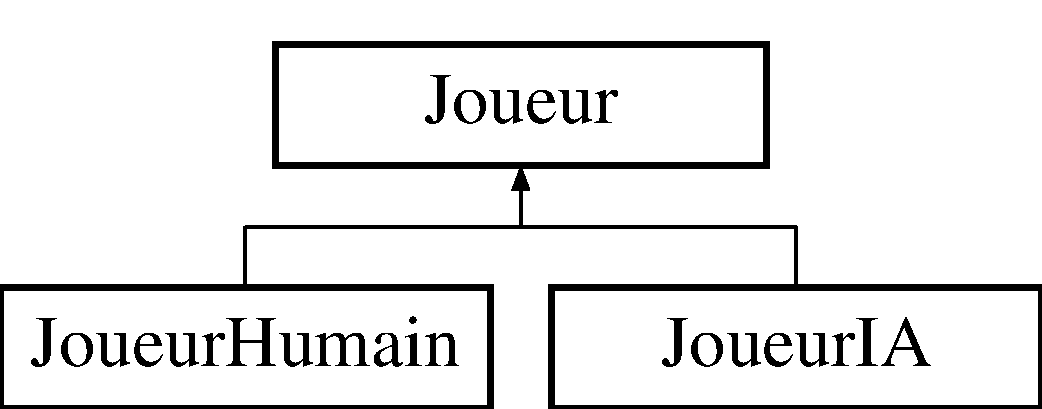
\includegraphics[height=2.000000cm]{class_joueur}
\end{center}
\end{figure}
\subsection*{Fonctions membres publiques}
\begin{DoxyCompactItemize}
\item 
\hyperlink{class_joueur_a951f6cb508b2d681eac4be586b8aac5f}{Joueur} ()\hypertarget{class_joueur_a951f6cb508b2d681eac4be586b8aac5f}{}\label{class_joueur_a951f6cb508b2d681eac4be586b8aac5f}

\begin{DoxyCompactList}\small\item\em Constructeur de la classe \hyperlink{class_joueur}{Joueur} qui met ses caractéristiques en ses valeurs par défaut. \end{DoxyCompactList}\item 
virtual bool \hyperlink{class_joueur_aee337662730df358b20474cac70d83e6}{est\+Une\+IA} ()
\begin{DoxyCompactList}\small\item\em Permet de savoir si ce joueur est une IA. Est utile lorsque l\textquotesingle{}on manipule un \hyperlink{class_joueur}{Joueur} et que l\textquotesingle{}on ne sait pas s\textquotesingle{}il est IA ou Humain. \end{DoxyCompactList}\item 
void \hyperlink{class_joueur_a07c1eba4f8531d594380fbcaaab240f6}{reset\+Grilles} ()\hypertarget{class_joueur_a07c1eba4f8531d594380fbcaaab240f6}{}\label{class_joueur_a07c1eba4f8531d594380fbcaaab240f6}

\begin{DoxyCompactList}\small\item\em fonction qui alloue la mémoire pour la grille et la grille des tentatives et les remplie de 0, donc d\textquotesingle{}eau \end{DoxyCompactList}\item 
void \hyperlink{class_joueur_a1f4357df61efbc2ead45d24a190ebb83}{definir\+Bateaux\+Type2} (int nb\+Max\+De\+Bateaux, int taille\+Grille)
\begin{DoxyCompactList}\small\item\em function permettant de définir un tableau de bateaux de tailles aléatoires \end{DoxyCompactList}\item 
void \hyperlink{class_joueur_a7f016748c27a4ddad2d363f4b5121ab1}{set\+Nom} (std\+::string nouveau\+Nom)
\begin{DoxyCompactList}\small\item\em fonction qui modifie l\textquotesingle{}attribut nom \end{DoxyCompactList}\item 
void \hyperlink{class_joueur_a424aec3294ea6019f372fd2d67ae5001}{set\+Grille} (char $\ast$$\ast$\hyperlink{class_joueur_a97a052f0b9966c94c49862df3144a62f}{grille}, int h, int l)
\begin{DoxyCompactList}\small\item\em fonction qui modifie les caractéristiques de la grille \end{DoxyCompactList}\item 
void \hyperlink{class_joueur_a11942778d97fd6f5823d8ef1ab964047}{set\+Grille\+Tentatives} (char $\ast$$\ast$\hyperlink{class_joueur_abbef5ee9c9c05a24ffa2c462e14cdfd7}{grille\+Tentatives})
\begin{DoxyCompactList}\small\item\em fonction qui modifie l\textquotesingle{}attribut grille\+Tentatives \end{DoxyCompactList}\item 
virtual void \hyperlink{class_joueur_a9027bfc622d9a175340b5fffe915c7b2}{demander\+Nom} ()\hypertarget{class_joueur_a9027bfc622d9a175340b5fffe915c7b2}{}\label{class_joueur_a9027bfc622d9a175340b5fffe915c7b2}

\begin{DoxyCompactList}\small\item\em initialise le nom du joueur en demandant le nom au joueur \end{DoxyCompactList}\item 
virtual void \hyperlink{class_joueur_a58fe79e4845404f361d5bc0fe9474135}{demander\+Taille\+Grille} ()\hypertarget{class_joueur_a58fe79e4845404f361d5bc0fe9474135}{}\label{class_joueur_a58fe79e4845404f361d5bc0fe9474135}

\begin{DoxyCompactList}\small\item\em initialise la taille de la grille en la demandant au joueur \end{DoxyCompactList}\item 
virtual char \hyperlink{class_joueur_a72fcb63683baba74922df5de246bff6f}{demander\+Type\+Jeu} ()\hypertarget{class_joueur_a72fcb63683baba74922df5de246bff6f}{}\label{class_joueur_a72fcb63683baba74922df5de246bff6f}

\begin{DoxyCompactList}\small\item\em fonction qui permet au joueur de choisir son type de jeu \+: bataille classique ou bataille améliorée \end{DoxyCompactList}\item 
virtual void \hyperlink{class_joueur_a5f0ab55bcb47e6808e46ef4515ce9565}{placement\+Des\+Bateaux} (char type\+Jeu)
\begin{DoxyCompactList}\small\item\em demande au joueur de placer ses différents bateaux. Utilise ajout\+Bateau pour chaqun des bateaux du joueur. \end{DoxyCompactList}\item 
virtual int $\ast$ \hyperlink{class_joueur_a46bdd92b73a1f0d04aeb5f19f33720b0}{tour} ()
\begin{DoxyCompactList}\small\item\em Permet de placer une bombe, affiche aussi la grille et la grille de tentatives. \end{DoxyCompactList}\item 
virtual void \hyperlink{class_joueur_a661426005c03ad2ee421249758f5c2a7}{resultat\+Bombe} (bool touche, int x, int y)
\begin{DoxyCompactList}\small\item\em Notifie le joueur si sa bombe a touché l\textquotesingle{}adversaire. \end{DoxyCompactList}\item 
virtual void \hyperlink{class_joueur_aeb9de0a7501a5370d45e670e122b3676}{resultat\+Bombe\+Adverse} (bool touche, int x, int y)
\begin{DoxyCompactList}\small\item\em Notifie le joueur si la bombe de l\textquotesingle{}adversaire l\textquotesingle{}a touché. \end{DoxyCompactList}\end{DoxyCompactItemize}
\subsection*{Fonctions membres protégées}
\begin{DoxyCompactItemize}
\item 
virtual void \hyperlink{class_joueur_a817129cc5062c058a153a241c74eee79}{placer\+Bateau} (\hyperlink{class_bateau}{Bateau} $\ast$b)
\begin{DoxyCompactList}\small\item\em Permet au joueur de positionner le bateau {\ttfamily $\ast$b} sur la grille. Cette fonction lui demande les coordonnées en x, y du bateau (en utilisant la fonction demander\+Coordonnees\+Bateau) mais aussi son orientation. \end{DoxyCompactList}\item 
void \hyperlink{class_joueur_ab42cd00f0ff47934eecde3fbaf06f2a5}{marquer\+Resultat\+Bombe\+Sur\+Grille\+Tentative} (bool touche, int x, int y)
\begin{DoxyCompactList}\small\item\em function permettant de modifier une case de la grille des tentatives sachant les conséquences de la bombe \end{DoxyCompactList}\item 
void \hyperlink{class_joueur_a3b77de3d2a5d2845bfefddb051460e80}{marquer\+Resultat\+Bombe\+Sur\+Grille} (bool touche, int x, int y)
\begin{DoxyCompactList}\small\item\em function permettant de modifier une case de la grille sachant les conséquences de la bombe \end{DoxyCompactList}\end{DoxyCompactItemize}
\subsection*{Attributs protégés}
\begin{DoxyCompactItemize}
\item 
std\+::string \hyperlink{class_joueur_abaee0b4f259181bf66dbab54bef971bb}{nom}
\item 
\hyperlink{class_grille}{Grille} \hyperlink{class_joueur_a97a052f0b9966c94c49862df3144a62f}{grille}
\item 
\hyperlink{class_grille}{Grille} \hyperlink{class_joueur_abbef5ee9c9c05a24ffa2c462e14cdfd7}{grille\+Tentatives}
\item 
int \hyperlink{class_joueur_a3a41069191547937ddd3acd15eecd4ee}{nb\+Cases\+Bateaux\+Touches}
\item 
int \hyperlink{class_joueur_a29e4485fe7b0a3f2c962757b7c7bf2a5}{nb\+Cases\+Bateaux}
\item 
int \hyperlink{class_joueur_a56752b0a96da94b17b07fd0312035a13}{nb\+Bateaux}
\item 
\hyperlink{class_bateau}{Bateau} $\ast$ \hyperlink{class_joueur_acf537ce482b493555318da7da14d8ac9}{bateaux}
\item 
\hyperlink{class_affichage}{Affichage} $\ast$ \hyperlink{class_joueur_a388634e5c242146dad447bc04756bab5}{affichage}
\end{DoxyCompactItemize}
\subsection*{Amis}
\begin{DoxyCompactItemize}
\item 
class {\bfseries Jeu\+Bataille\+Navale}\hypertarget{class_joueur_a5e820295bb9a9381c14f9067e97ca6c1}{}\label{class_joueur_a5e820295bb9a9381c14f9067e97ca6c1}

\end{DoxyCompactItemize}


\subsection{Description détaillée}
classe \hyperlink{class_joueur}{Joueur} regroupant les fonctionnalités générales sur le joueur 

\subsection{Documentation des fonctions membres}
\index{Joueur@{Joueur}!definir\+Bateaux\+Type2@{definir\+Bateaux\+Type2}}
\index{definir\+Bateaux\+Type2@{definir\+Bateaux\+Type2}!Joueur@{Joueur}}
\subsubsection[{\texorpdfstring{definir\+Bateaux\+Type2(int nb\+Max\+De\+Bateaux, int taille\+Grille)}{definirBateauxType2(int nbMaxDeBateaux, int tailleGrille)}}]{\setlength{\rightskip}{0pt plus 5cm}public Joueur\+::definir\+Bateaux\+Type2 (
\begin{DoxyParamCaption}
\item[{int}]{nb\+Max\+De\+Bateaux, }
\item[{int}]{taille\+Grille}
\end{DoxyParamCaption}
)}\hypertarget{class_joueur_a1f4357df61efbc2ead45d24a190ebb83}{}\label{class_joueur_a1f4357df61efbc2ead45d24a190ebb83}


function permettant de définir un tableau de bateaux de tailles aléatoires 


\begin{DoxyParams}{Paramètres}
{\em nb\+Max\+De\+Bateaux,taille\+Grille} & le nombre de bateaux du tableau et la taille de la grille \\
\hline
\end{DoxyParams}
\index{Joueur@{Joueur}!est\+Une\+IA@{est\+Une\+IA}}
\index{est\+Une\+IA@{est\+Une\+IA}!Joueur@{Joueur}}
\subsubsection[{\texorpdfstring{est\+Une\+I\+A()}{estUneIA()}}]{\setlength{\rightskip}{0pt plus 5cm}public Joueur\+::est\+Une\+IA (
\begin{DoxyParamCaption}
{}
\end{DoxyParamCaption}
)\hspace{0.3cm}{\ttfamily [inline]}, {\ttfamily [virtual]}}\hypertarget{class_joueur_aee337662730df358b20474cac70d83e6}{}\label{class_joueur_aee337662730df358b20474cac70d83e6}


Permet de savoir si ce joueur est une IA. Est utile lorsque l\textquotesingle{}on manipule un \hyperlink{class_joueur}{Joueur} et que l\textquotesingle{}on ne sait pas s\textquotesingle{}il est IA ou Humain. 

\begin{DoxyReturn}{Renvoie}
true si c\textquotesingle{}est une IA, false sinon. 
\end{DoxyReturn}


Réimplémentée dans \hyperlink{class_joueur_i_a_a549e94b2b4673dcf97041add34bc49a0}{Joueur\+IA}, et \hyperlink{class_joueur_humain_a4d531faca2e5f81966ff11309bd1fd9e}{Joueur\+Humain}.

\index{Joueur@{Joueur}!marquer\+Resultat\+Bombe\+Sur\+Grille@{marquer\+Resultat\+Bombe\+Sur\+Grille}}
\index{marquer\+Resultat\+Bombe\+Sur\+Grille@{marquer\+Resultat\+Bombe\+Sur\+Grille}!Joueur@{Joueur}}
\subsubsection[{\texorpdfstring{marquer\+Resultat\+Bombe\+Sur\+Grille(bool touche, int x, int y)}{marquerResultatBombeSurGrille(bool touche, int x, int y)}}]{\setlength{\rightskip}{0pt plus 5cm}protected Joueur\+::marquer\+Resultat\+Bombe\+Sur\+Grille (
\begin{DoxyParamCaption}
\item[{bool}]{touche, }
\item[{int}]{x, }
\item[{int}]{y}
\end{DoxyParamCaption}
)\hspace{0.3cm}{\ttfamily [protected]}}\hypertarget{class_joueur_a3b77de3d2a5d2845bfefddb051460e80}{}\label{class_joueur_a3b77de3d2a5d2845bfefddb051460e80}


function permettant de modifier une case de la grille sachant les conséquences de la bombe 


\begin{DoxyParams}{Paramètres}
{\em touche,x,y} & les coordonnées de la position à modifier, et touche\+: l\textquotesingle{}indication si la bombe a atteint sa cible \\
\hline
\end{DoxyParams}
\index{Joueur@{Joueur}!marquer\+Resultat\+Bombe\+Sur\+Grille\+Tentative@{marquer\+Resultat\+Bombe\+Sur\+Grille\+Tentative}}
\index{marquer\+Resultat\+Bombe\+Sur\+Grille\+Tentative@{marquer\+Resultat\+Bombe\+Sur\+Grille\+Tentative}!Joueur@{Joueur}}
\subsubsection[{\texorpdfstring{marquer\+Resultat\+Bombe\+Sur\+Grille\+Tentative(bool touche, int x, int y)}{marquerResultatBombeSurGrilleTentative(bool touche, int x, int y)}}]{\setlength{\rightskip}{0pt plus 5cm}protected Joueur\+::marquer\+Resultat\+Bombe\+Sur\+Grille\+Tentative (
\begin{DoxyParamCaption}
\item[{bool}]{touche, }
\item[{int}]{x, }
\item[{int}]{y}
\end{DoxyParamCaption}
)\hspace{0.3cm}{\ttfamily [protected]}}\hypertarget{class_joueur_ab42cd00f0ff47934eecde3fbaf06f2a5}{}\label{class_joueur_ab42cd00f0ff47934eecde3fbaf06f2a5}


function permettant de modifier une case de la grille des tentatives sachant les conséquences de la bombe 


\begin{DoxyParams}{Paramètres}
{\em touche,x,y} & les coordonnées de la position à modifier, et touche\+: l\textquotesingle{}indication si la bombe a atteint sa cible \\
\hline
\end{DoxyParams}
\index{Joueur@{Joueur}!placement\+Des\+Bateaux@{placement\+Des\+Bateaux}}
\index{placement\+Des\+Bateaux@{placement\+Des\+Bateaux}!Joueur@{Joueur}}
\subsubsection[{\texorpdfstring{placement\+Des\+Bateaux(char type\+Jeu)}{placementDesBateaux(char typeJeu)}}]{\setlength{\rightskip}{0pt plus 5cm}public Joueur\+::placement\+Des\+Bateaux (
\begin{DoxyParamCaption}
\item[{char}]{type\+Jeu}
\end{DoxyParamCaption}
)\hspace{0.3cm}{\ttfamily [inline]}, {\ttfamily [virtual]}}\hypertarget{class_joueur_a5f0ab55bcb47e6808e46ef4515ce9565}{}\label{class_joueur_a5f0ab55bcb47e6808e46ef4515ce9565}


demande au joueur de placer ses différents bateaux. Utilise ajout\+Bateau pour chaqun des bateaux du joueur. 


\begin{DoxyParams}{Paramètres}
{\em type\+Jeu} & le type de jeu choisis \\
\hline
\end{DoxyParams}


Réimplémentée dans \hyperlink{class_joueur_i_a_a6d7592fa8c653cb5420270d61467419b}{Joueur\+IA}, et \hyperlink{class_joueur_humain_ae27bf69ba0db87cd8268ba1cd1e4f817}{Joueur\+Humain}.

\index{Joueur@{Joueur}!placer\+Bateau@{placer\+Bateau}}
\index{placer\+Bateau@{placer\+Bateau}!Joueur@{Joueur}}
\subsubsection[{\texorpdfstring{placer\+Bateau(\+Bateau $\ast$b)}{placerBateau(Bateau *b)}}]{\setlength{\rightskip}{0pt plus 5cm}protected Joueur\+::placer\+Bateau (
\begin{DoxyParamCaption}
\item[{{\bf Bateau} $\ast$}]{b}
\end{DoxyParamCaption}
)\hspace{0.3cm}{\ttfamily [inline]}, {\ttfamily [protected]}, {\ttfamily [virtual]}}\hypertarget{class_joueur_a817129cc5062c058a153a241c74eee79}{}\label{class_joueur_a817129cc5062c058a153a241c74eee79}


Permet au joueur de positionner le bateau {\ttfamily $\ast$b} sur la grille. Cette fonction lui demande les coordonnées en x, y du bateau (en utilisant la fonction demander\+Coordonnees\+Bateau) mais aussi son orientation. 


\begin{DoxyParams}{Paramètres}
{\em $\ast$b} & Un pointeur sur le bateau que le joueur va placer sur la grille. \\
\hline
\end{DoxyParams}


Réimplémentée dans \hyperlink{class_joueur_humain_af9e3ccafc7cde958dda81551d0ef6abd}{Joueur\+Humain}, et \hyperlink{class_joueur_i_a_a70a56322ca6eeeb52612510d7e22d388}{Joueur\+IA}.

\index{Joueur@{Joueur}!resultat\+Bombe@{resultat\+Bombe}}
\index{resultat\+Bombe@{resultat\+Bombe}!Joueur@{Joueur}}
\subsubsection[{\texorpdfstring{resultat\+Bombe(bool touche, int x, int y)}{resultatBombe(bool touche, int x, int y)}}]{\setlength{\rightskip}{0pt plus 5cm}public Joueur\+::resultat\+Bombe (
\begin{DoxyParamCaption}
\item[{bool}]{touche, }
\item[{int}]{x, }
\item[{int}]{y}
\end{DoxyParamCaption}
)\hspace{0.3cm}{\ttfamily [inline]}, {\ttfamily [virtual]}}\hypertarget{class_joueur_a661426005c03ad2ee421249758f5c2a7}{}\label{class_joueur_a661426005c03ad2ee421249758f5c2a7}


Notifie le joueur si sa bombe a touché l\textquotesingle{}adversaire. 


\begin{DoxyParams}{Paramètres}
{\em touche} & true si la bombe a touché un navire adverse, false sinon. \\
\hline
{\em x} & La coordonnée en x de la bombe que le joueur avait choisie. \\
\hline
{\em y} & La coordonnée en y de la bombe que le joueur avait choisie. \\
\hline
\end{DoxyParams}


Réimplémentée dans \hyperlink{class_joueur_i_a_a5e7ed6369200fe44382a54cf739ad8b3}{Joueur\+IA}, et \hyperlink{class_joueur_humain_a9eeae3b54b174e477a94c75d57a0d403}{Joueur\+Humain}.

\index{Joueur@{Joueur}!resultat\+Bombe\+Adverse@{resultat\+Bombe\+Adverse}}
\index{resultat\+Bombe\+Adverse@{resultat\+Bombe\+Adverse}!Joueur@{Joueur}}
\subsubsection[{\texorpdfstring{resultat\+Bombe\+Adverse(bool touche, int x, int y)}{resultatBombeAdverse(bool touche, int x, int y)}}]{\setlength{\rightskip}{0pt plus 5cm}public Joueur\+::resultat\+Bombe\+Adverse (
\begin{DoxyParamCaption}
\item[{bool}]{touche, }
\item[{int}]{x, }
\item[{int}]{y}
\end{DoxyParamCaption}
)\hspace{0.3cm}{\ttfamily [inline]}, {\ttfamily [virtual]}}\hypertarget{class_joueur_aeb9de0a7501a5370d45e670e122b3676}{}\label{class_joueur_aeb9de0a7501a5370d45e670e122b3676}


Notifie le joueur si la bombe de l\textquotesingle{}adversaire l\textquotesingle{}a touché. 


\begin{DoxyParams}{Paramètres}
{\em touche} & true si la bombe a touché un navire, false sinon. \\
\hline
{\em x} & La coordonnée en x de la bombe que le joueur adverse avait choisie. \\
\hline
{\em y} & La coordonnée en y de la bombe que le joueur adverse avait choisie. \\
\hline
\end{DoxyParams}


Réimplémentée dans \hyperlink{class_joueur_i_a_a35dfe27baa0fb62a927cc13186b09920}{Joueur\+IA}, et \hyperlink{class_joueur_humain_acdd6b332153e1543d083d272fbdf8289}{Joueur\+Humain}.

\index{Joueur@{Joueur}!set\+Grille@{set\+Grille}}
\index{set\+Grille@{set\+Grille}!Joueur@{Joueur}}
\subsubsection[{\texorpdfstring{set\+Grille(char $\ast$$\ast$grille, int h, int l)}{setGrille(char **grille, int h, int l)}}]{\setlength{\rightskip}{0pt plus 5cm}public Joueur\+::set\+Grille (
\begin{DoxyParamCaption}
\item[{char $\ast$$\ast$}]{grille, }
\item[{int}]{h, }
\item[{int}]{l}
\end{DoxyParamCaption}
)}\hypertarget{class_joueur_a424aec3294ea6019f372fd2d67ae5001}{}\label{class_joueur_a424aec3294ea6019f372fd2d67ae5001}


fonction qui modifie les caractéristiques de la grille 


\begin{DoxyParams}{Paramètres}
{\em grille,h,l} & grille\+: object modifié, hauteur, largueur \\
\hline
\end{DoxyParams}
\index{Joueur@{Joueur}!set\+Grille\+Tentatives@{set\+Grille\+Tentatives}}
\index{set\+Grille\+Tentatives@{set\+Grille\+Tentatives}!Joueur@{Joueur}}
\subsubsection[{\texorpdfstring{set\+Grille\+Tentatives(char $\ast$$\ast$grille\+Tentatives)}{setGrilleTentatives(char **grilleTentatives)}}]{\setlength{\rightskip}{0pt plus 5cm}public Joueur\+::set\+Grille\+Tentatives (
\begin{DoxyParamCaption}
\item[{char $\ast$$\ast$}]{grille\+Tentatives}
\end{DoxyParamCaption}
)}\hypertarget{class_joueur_a11942778d97fd6f5823d8ef1ab964047}{}\label{class_joueur_a11942778d97fd6f5823d8ef1ab964047}


fonction qui modifie l\textquotesingle{}attribut grille\+Tentatives 


\begin{DoxyParams}{Paramètres}
{\em $\ast$$\ast$grille\+Tentatives} & \\
\hline
\end{DoxyParams}
\index{Joueur@{Joueur}!set\+Nom@{set\+Nom}}
\index{set\+Nom@{set\+Nom}!Joueur@{Joueur}}
\subsubsection[{\texorpdfstring{set\+Nom(std\+::string nouveau\+Nom)}{setNom(std::string nouveauNom)}}]{\setlength{\rightskip}{0pt plus 5cm}public Joueur\+::set\+Nom (
\begin{DoxyParamCaption}
\item[{std\+::string}]{nouveau\+Nom}
\end{DoxyParamCaption}
)}\hypertarget{class_joueur_a7f016748c27a4ddad2d363f4b5121ab1}{}\label{class_joueur_a7f016748c27a4ddad2d363f4b5121ab1}


fonction qui modifie l\textquotesingle{}attribut nom 


\begin{DoxyParams}{Paramètres}
{\em nouveau\+Nom} & \\
\hline
\end{DoxyParams}
\index{Joueur@{Joueur}!tour@{tour}}
\index{tour@{tour}!Joueur@{Joueur}}
\subsubsection[{\texorpdfstring{tour()}{tour()}}]{\setlength{\rightskip}{0pt plus 5cm}public Joueur\+::tour (
\begin{DoxyParamCaption}
{}
\end{DoxyParamCaption}
)\hspace{0.3cm}{\ttfamily [inline]}, {\ttfamily [virtual]}}\hypertarget{class_joueur_a46bdd92b73a1f0d04aeb5f19f33720b0}{}\label{class_joueur_a46bdd92b73a1f0d04aeb5f19f33720b0}


Permet de placer une bombe, affiche aussi la grille et la grille de tentatives. 

\begin{DoxyReturn}{Renvoie}
Les coordonnées de la bombe cible. Sous la forme d\textquotesingle{}un tableau \mbox{[}x, y\mbox{]}. 
\end{DoxyReturn}


Réimplémentée dans \hyperlink{class_joueur_i_a_a76b3e9af59c86acb34d7e1cb70802436}{Joueur\+IA}, et \hyperlink{class_joueur_humain_a92f4cb99ff2957813da34fb60e211870}{Joueur\+Humain}.



\subsection{Documentation des données membres}
\index{Joueur@{Joueur}!affichage@{affichage}}
\index{affichage@{affichage}!Joueur@{Joueur}}
\subsubsection[{\texorpdfstring{affichage}{affichage}}]{\setlength{\rightskip}{0pt plus 5cm}{\bf Affichage}$\ast$ Joueur\+::affichage\hspace{0.3cm}{\ttfamily [protected]}}\hypertarget{class_joueur_a388634e5c242146dad447bc04756bab5}{}\label{class_joueur_a388634e5c242146dad447bc04756bab5}
Un affichage pour afficher des informations générales sur le jeux. \index{Joueur@{Joueur}!bateaux@{bateaux}}
\index{bateaux@{bateaux}!Joueur@{Joueur}}
\subsubsection[{\texorpdfstring{bateaux}{bateaux}}]{\setlength{\rightskip}{0pt plus 5cm}{\bf Bateau}$\ast$ Joueur\+::bateaux\hspace{0.3cm}{\ttfamily [protected]}}\hypertarget{class_joueur_acf537ce482b493555318da7da14d8ac9}{}\label{class_joueur_acf537ce482b493555318da7da14d8ac9}
Un tableau contenant les bateaux possédés par le joueur et qu\textquotesingle{}il a placé sur la grille. \index{Joueur@{Joueur}!grille@{grille}}
\index{grille@{grille}!Joueur@{Joueur}}
\subsubsection[{\texorpdfstring{grille}{grille}}]{\setlength{\rightskip}{0pt plus 5cm}{\bf Grille} Joueur\+::grille\hspace{0.3cm}{\ttfamily [protected]}}\hypertarget{class_joueur_a97a052f0b9966c94c49862df3144a62f}{}\label{class_joueur_a97a052f0b9966c94c49862df3144a62f}
La grille sur laquelle le joueur place ses bateaux \index{Joueur@{Joueur}!grille\+Tentatives@{grille\+Tentatives}}
\index{grille\+Tentatives@{grille\+Tentatives}!Joueur@{Joueur}}
\subsubsection[{\texorpdfstring{grille\+Tentatives}{grilleTentatives}}]{\setlength{\rightskip}{0pt plus 5cm}{\bf Grille} Joueur\+::grille\+Tentatives\hspace{0.3cm}{\ttfamily [protected]}}\hypertarget{class_joueur_abbef5ee9c9c05a24ffa2c462e14cdfd7}{}\label{class_joueur_abbef5ee9c9c05a24ffa2c462e14cdfd7}
La grille permettant de garder en mémoire les tentatives de bombes effectuées par le joueur \index{Joueur@{Joueur}!nb\+Bateaux@{nb\+Bateaux}}
\index{nb\+Bateaux@{nb\+Bateaux}!Joueur@{Joueur}}
\subsubsection[{\texorpdfstring{nb\+Bateaux}{nbBateaux}}]{\setlength{\rightskip}{0pt plus 5cm}int Joueur\+::nb\+Bateaux\hspace{0.3cm}{\ttfamily [protected]}}\hypertarget{class_joueur_a56752b0a96da94b17b07fd0312035a13}{}\label{class_joueur_a56752b0a96da94b17b07fd0312035a13}
/ Le nombre de bateau initial du joueur. Permet de simplifier l\textquotesingle{}écriture de certaines boucles. ( i $<$ nb\+Bateaux etc) \index{Joueur@{Joueur}!nb\+Cases\+Bateaux@{nb\+Cases\+Bateaux}}
\index{nb\+Cases\+Bateaux@{nb\+Cases\+Bateaux}!Joueur@{Joueur}}
\subsubsection[{\texorpdfstring{nb\+Cases\+Bateaux}{nbCasesBateaux}}]{\setlength{\rightskip}{0pt plus 5cm}int Joueur\+::nb\+Cases\+Bateaux\hspace{0.3cm}{\ttfamily [protected]}}\hypertarget{class_joueur_a29e4485fe7b0a3f2c962757b7c7bf2a5}{}\label{class_joueur_a29e4485fe7b0a3f2c962757b7c7bf2a5}
Le nombre de cases occupées par des bateaux sur la grille \index{Joueur@{Joueur}!nb\+Cases\+Bateaux\+Touches@{nb\+Cases\+Bateaux\+Touches}}
\index{nb\+Cases\+Bateaux\+Touches@{nb\+Cases\+Bateaux\+Touches}!Joueur@{Joueur}}
\subsubsection[{\texorpdfstring{nb\+Cases\+Bateaux\+Touches}{nbCasesBateauxTouches}}]{\setlength{\rightskip}{0pt plus 5cm}int Joueur\+::nb\+Cases\+Bateaux\+Touches\hspace{0.3cm}{\ttfamily [protected]}}\hypertarget{class_joueur_a3a41069191547937ddd3acd15eecd4ee}{}\label{class_joueur_a3a41069191547937ddd3acd15eecd4ee}
Correspond au nombre de fois que l\textquotesingle{}adversaire a touché un bateau.\+Va être incrementé quand un des bateaux est touché pour faciliter la vérification de la fin de partie. \index{Joueur@{Joueur}!nom@{nom}}
\index{nom@{nom}!Joueur@{Joueur}}
\subsubsection[{\texorpdfstring{nom}{nom}}]{\setlength{\rightskip}{0pt plus 5cm}std\+::string Joueur\+::nom\hspace{0.3cm}{\ttfamily [protected]}}\hypertarget{class_joueur_abaee0b4f259181bf66dbab54bef971bb}{}\label{class_joueur_abaee0b4f259181bf66dbab54bef971bb}
Le nom du joueur 

La documentation de cette classe a été générée à partir des fichiers suivants \+:\begin{DoxyCompactItemize}
\item 
/home/lucas/\+Documents/\+Git\+Hub/\+Bataille-\/\+Navale/src/\hyperlink{_joueur_8hpp}{Joueur.\+hpp}\item 
/home/lucas/\+Documents/\+Git\+Hub/\+Bataille-\/\+Navale/src/Joueur.\+cpp\end{DoxyCompactItemize}

\hypertarget{class_joueur_humain}{}\section{Référence de la classe Joueur\+Humain}
\label{class_joueur_humain}\index{Joueur\+Humain@{Joueur\+Humain}}


classe representant le joueur qui est humain. Cette classe hérite de la classe \hyperlink{class_joueur}{Joueur}  




{\ttfamily \#include $<$Joueur\+Humain.\+hpp$>$}

Graphe d\textquotesingle{}héritage de Joueur\+Humain\+:\begin{figure}[H]
\begin{center}
\leavevmode
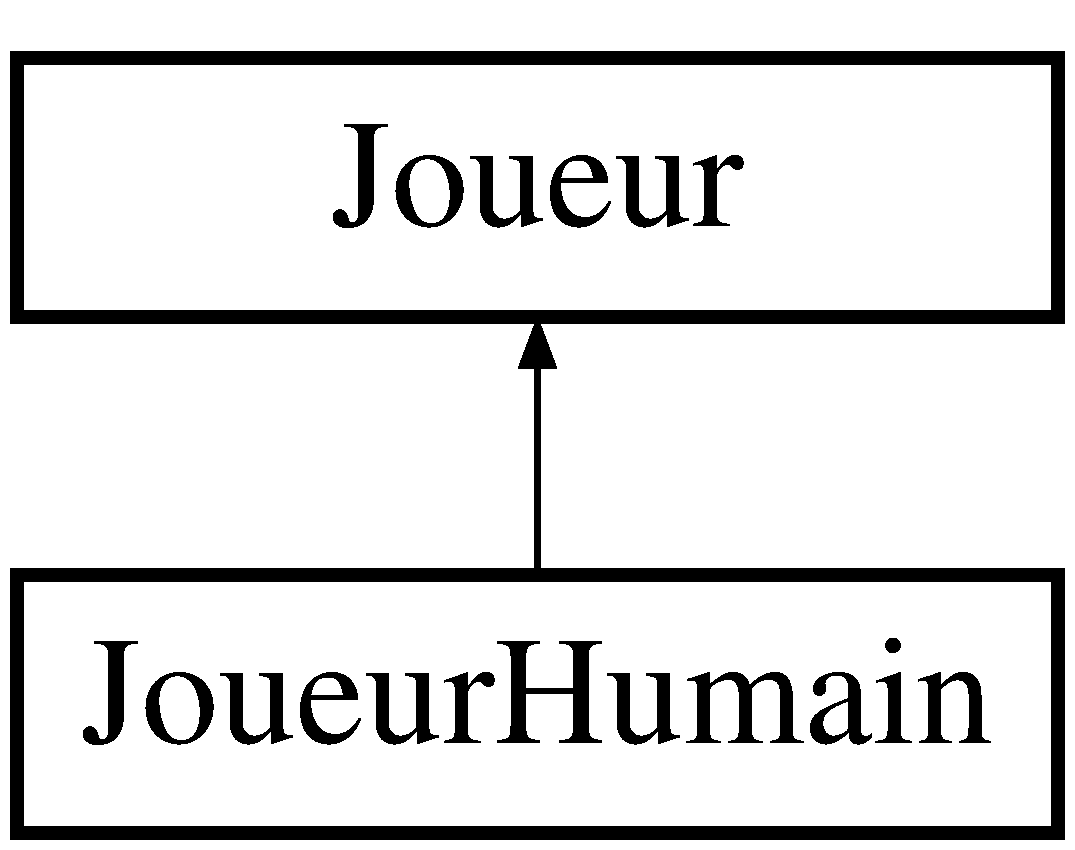
\includegraphics[height=2.000000cm]{class_joueur_humain}
\end{center}
\end{figure}
\subsection*{Fonctions membres publiques}
\begin{DoxyCompactItemize}
\item 
virtual void \hyperlink{class_joueur_humain_afde5ace70d8664257e7774beea718120}{demander\+Nom} ()\hypertarget{class_joueur_humain_afde5ace70d8664257e7774beea718120}{}\label{class_joueur_humain_afde5ace70d8664257e7774beea718120}

\begin{DoxyCompactList}\small\item\em initialise le nom du joueur en demandant le nom au joueur \end{DoxyCompactList}\item 
virtual void {\bfseries demander\+Taille\+Grille} ()\hypertarget{class_joueur_humain_aecd25abe7629ee3925004e2f0bcb7c7e}{}\label{class_joueur_humain_aecd25abe7629ee3925004e2f0bcb7c7e}

\item 
virtual char {\bfseries demander\+Type\+Jeu} ()\hypertarget{class_joueur_humain_a63677d4f1eb52cfa30d932a78098aee7}{}\label{class_joueur_humain_a63677d4f1eb52cfa30d932a78098aee7}

\item 
virtual void \hyperlink{class_joueur_humain_a31e23d1e076b0e6110e0a9d354d80674}{placement\+Des\+Bateaux} (char type\+Jeu)
\begin{DoxyCompactList}\small\item\em demande au joueur de placer ses différents bateaux. Utilise ajout\+Bateau pour chaqun des bateaux du joueur. \end{DoxyCompactList}\end{DoxyCompactItemize}
\subsection*{Fonctions membres privées}
\begin{DoxyCompactItemize}
\item 
virtual void {\bfseries placer\+Bateau} (Bateau $\ast$b)\hypertarget{class_joueur_humain_a12d0d611801d881138d9af0ca8e219c8}{}\label{class_joueur_humain_a12d0d611801d881138d9af0ca8e219c8}

\item 
void {\bfseries demander\+Coordonnees\+Bateau} (Bateau $\ast$b)\hypertarget{class_joueur_humain_aee35cac62f530e2ba30663853c87646d}{}\label{class_joueur_humain_aee35cac62f530e2ba30663853c87646d}

\end{DoxyCompactItemize}
\subsection*{Membres hérités additionnels}


\subsection{Description détaillée}
classe representant le joueur qui est humain. Cette classe hérite de la classe \hyperlink{class_joueur}{Joueur} 

La classe gere les actions du joueur. 

\subsection{Documentation des fonctions membres}
\index{Joueur\+Humain@{Joueur\+Humain}!placement\+Des\+Bateaux@{placement\+Des\+Bateaux}}
\index{placement\+Des\+Bateaux@{placement\+Des\+Bateaux}!Joueur\+Humain@{Joueur\+Humain}}
\subsubsection[{\texorpdfstring{placement\+Des\+Bateaux(char type\+Jeu)}{placementDesBateaux(char typeJeu)}}]{\setlength{\rightskip}{0pt plus 5cm}void Joueur\+Humain\+::placement\+Des\+Bateaux (
\begin{DoxyParamCaption}
\item[{char}]{type\+Jeu}
\end{DoxyParamCaption}
)\hspace{0.3cm}{\ttfamily [virtual]}}\hypertarget{class_joueur_humain_a31e23d1e076b0e6110e0a9d354d80674}{}\label{class_joueur_humain_a31e23d1e076b0e6110e0a9d354d80674}


demande au joueur de placer ses différents bateaux. Utilise ajout\+Bateau pour chaqun des bateaux du joueur. 


\begin{DoxyParams}{Paramètres}
{\em type\+Jeu} & le type de jeu choisis \\
\hline
\end{DoxyParams}


Réimplémentée à partir de \hyperlink{class_joueur_aa97f71a90328693e0047ba2f48d61b4b}{Joueur}.



La documentation de cette classe a été générée à partir des fichiers suivants \+:\begin{DoxyCompactItemize}
\item 
/home/lucas/\+Documents/\+Git\+Hub/\+Bataille-\/\+Navale/src/\hyperlink{_joueur_humain_8hpp}{Joueur\+Humain.\+hpp}\item 
/home/lucas/\+Documents/\+Git\+Hub/\+Bataille-\/\+Navale/src/Joueur\+Humain.\+cpp\end{DoxyCompactItemize}

\hypertarget{class_joueur_i_a}{}\section{Référence de la classe Joueur\+IA}
\label{class_joueur_i_a}\index{Joueur\+IA@{Joueur\+IA}}


classe representant le joueur qui est IA. Cette classe hérite de la classe \hyperlink{class_joueur}{Joueur}  




{\ttfamily \#include $<$Joueur\+I\+A.\+hpp$>$}

Graphe d\textquotesingle{}héritage de Joueur\+IA\+:\begin{figure}[H]
\begin{center}
\leavevmode
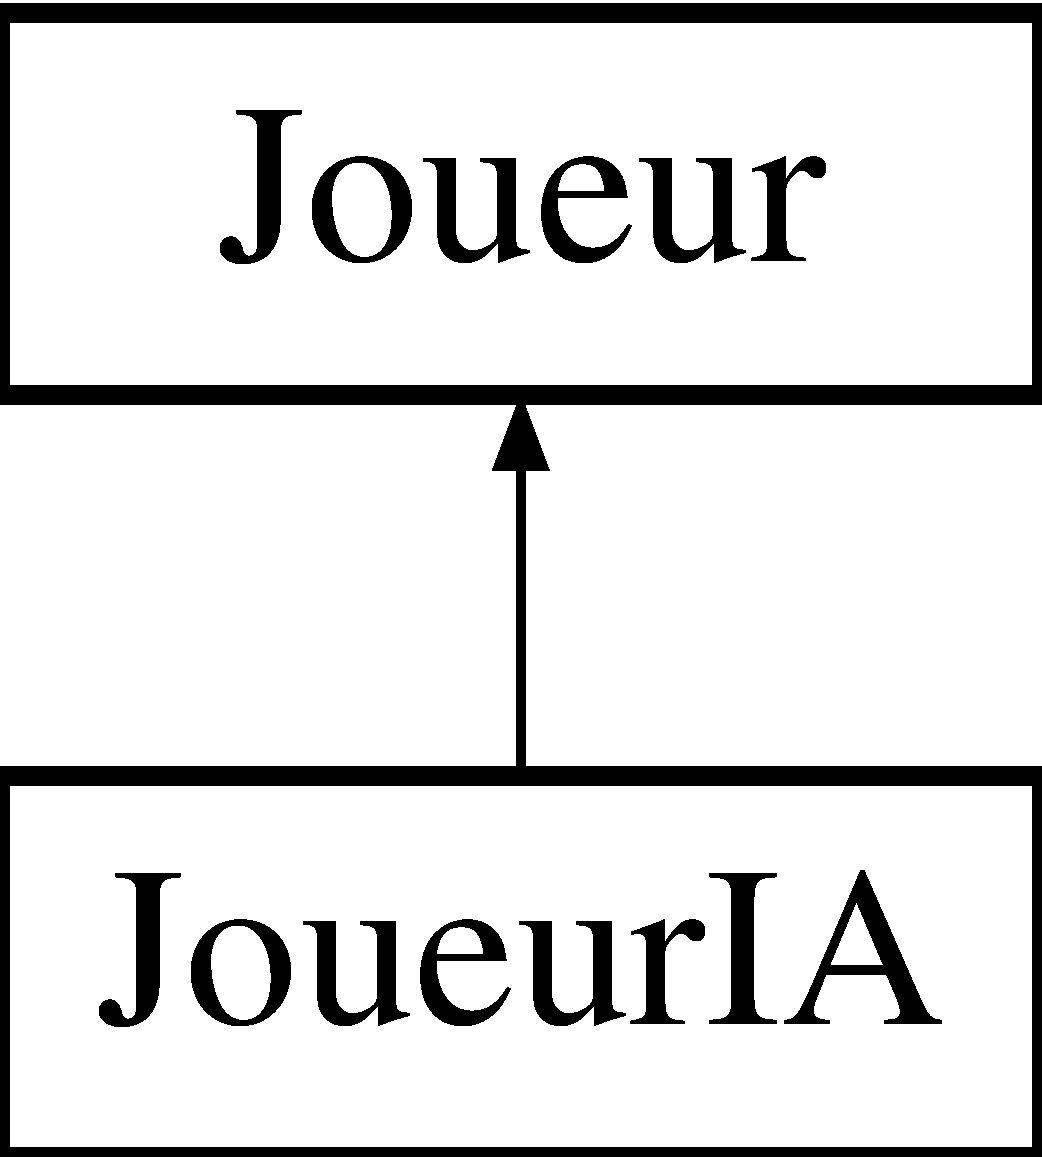
\includegraphics[height=2.000000cm]{class_joueur_i_a}
\end{center}
\end{figure}
\subsection*{Fonctions membres publiques}
\begin{DoxyCompactItemize}
\item 
\hyperlink{class_joueur_i_a_a88187887d491910b2e7e969fb9ea4188}{Joueur\+IA} ()\hypertarget{class_joueur_i_a_a88187887d491910b2e7e969fb9ea4188}{}\label{class_joueur_i_a_a88187887d491910b2e7e969fb9ea4188}

\begin{DoxyCompactList}\small\item\em Constructeur de \hyperlink{class_joueur_i_a}{Joueur\+IA}. \end{DoxyCompactList}\item 
virtual bool \hyperlink{class_joueur_i_a_a549e94b2b4673dcf97041add34bc49a0}{est\+Une\+IA} ()
\begin{DoxyCompactList}\small\item\em Permet de savoir si ce joueur est une IA. Est utile lorsque l\textquotesingle{}on manipule un \hyperlink{class_joueur}{Joueur} et que l\textquotesingle{}on ne sait pas s\textquotesingle{}il est IA ou Humain. \end{DoxyCompactList}\item 
virtual void \hyperlink{class_joueur_i_a_ac61e1573c44426a797fcd826ad21e03c}{demander\+Nom} ()\hypertarget{class_joueur_i_a_ac61e1573c44426a797fcd826ad21e03c}{}\label{class_joueur_i_a_ac61e1573c44426a797fcd826ad21e03c}

\begin{DoxyCompactList}\small\item\em L\textquotesingle{}IA donnera \char`\"{}\+I\+A\char`\"{} comme nom. \end{DoxyCompactList}\item 
virtual void \hyperlink{class_joueur_i_a_a073f19ae34a403f4d3bd70e5e82347a0}{demander\+Taille\+Grille} ()\hypertarget{class_joueur_i_a_a073f19ae34a403f4d3bd70e5e82347a0}{}\label{class_joueur_i_a_a073f19ae34a403f4d3bd70e5e82347a0}

\begin{DoxyCompactList}\small\item\em L\textquotesingle{}IA donnera toujours 10x10 comme taille de grille. \end{DoxyCompactList}\item 
virtual char \hyperlink{class_joueur_i_a_a3812f9bf6f315236286ea5ebad576a4f}{demander\+Type\+Jeu} ()
\begin{DoxyCompactList}\small\item\em L\textquotesingle{}IA donnera toujours un jeu de type 2. \end{DoxyCompactList}\item 
virtual void \hyperlink{class_joueur_i_a_a6d7592fa8c653cb5420270d61467419b}{placement\+Des\+Bateaux} (char type\+Jeu)
\begin{DoxyCompactList}\small\item\em Permet à l\textquotesingle{}IA de placer tous ses bateaux sur la grille. L\textquotesingle{}IA choisit d\textquotesingle{}abord de façon aléatoire quels bateaux elle va placer. Puis fais appel à la fonction \hyperlink{class_joueur_i_a_a70a56322ca6eeeb52612510d7e22d388}{placer\+Bateau(\+Bateau $\ast$b)}. \end{DoxyCompactList}\item 
virtual int $\ast$ \hyperlink{class_joueur_i_a_a76b3e9af59c86acb34d7e1cb70802436}{tour} ()
\begin{DoxyCompactList}\small\item\em Permet à l\textquotesingle{}IA de placer une bombe. Lui affiche aussi sa grille et sa grille de tentatives. Les coordonnées de la bombe sont déterminées à l\textquotesingle{}aide d\textquotesingle{}une fonction comme \hyperlink{class_joueur_i_a_af67d4959a40d9e99f0f8d99eaaf73c49}{determiner\+Coordonnees\+Bombes\+Scan()} ou \hyperlink{class_joueur_i_a_ad1fa6503f6fce1560129ee8cb94a1475}{determiner\+Coordonnees\+Bombes\+Aleatoire()}. \end{DoxyCompactList}\item 
virtual void \hyperlink{class_joueur_i_a_a5e7ed6369200fe44382a54cf739ad8b3}{resultat\+Bombe} (bool touche, int x, int y)
\begin{DoxyCompactList}\small\item\em Notifie l\textquotesingle{}IA si sa bombe a touché l\textquotesingle{}adversaire. On modifie alors sa grille en conséquence. \end{DoxyCompactList}\item 
virtual void \hyperlink{class_joueur_i_a_a35dfe27baa0fb62a927cc13186b09920}{resultat\+Bombe\+Adverse} (bool touche, int x, int y)
\begin{DoxyCompactList}\small\item\em Notifie l\textquotesingle{}IA si la bombe de l\textquotesingle{}adversaire l\textquotesingle{}a touché. \end{DoxyCompactList}\end{DoxyCompactItemize}
\subsection*{Fonctions membres privées}
\begin{DoxyCompactItemize}
\item 
virtual void \hyperlink{class_joueur_i_a_a70a56322ca6eeeb52612510d7e22d388}{placer\+Bateau} (\hyperlink{class_bateau}{Bateau} $\ast$bateau)
\begin{DoxyCompactList}\small\item\em Permet au joueur de positionner le bateau {\ttfamily $\ast$b} sur la grille. Cette fonction lui génère les coordonnées en x, y du bateau et son orientation. \end{DoxyCompactList}\item 
int $\ast$ \hyperlink{class_joueur_i_a_a83b8a54bbc3d6fad8fbdaee79a5a8246}{retirer\+De\+La\+Liste} (int $\ast$liste, int taille, int ind)
\begin{DoxyCompactList}\small\item\em Retire la valeur présente à l\textquotesingle{}indice {\ttfamily ind} de la liste {\ttfamily liste}. Il s\textquotesingle{}agit d\textquotesingle{}une liste d\textquotesingle{}indices correspondant aux bateaux que l\textquotesingle{}IA peut choisir. Cette liste est utilisée dans \hyperlink{class_joueur_i_a_a6d7592fa8c653cb5420270d61467419b}{placement\+Des\+Bateaux(char type\+Jeu)} \end{DoxyCompactList}\item 
int $\ast$ \hyperlink{class_joueur_i_a_ad1fa6503f6fce1560129ee8cb94a1475}{determiner\+Coordonnees\+Bombes\+Aleatoire} ()
\begin{DoxyCompactList}\small\item\em L\textquotesingle{}IA choisit d\textquotesingle{}envoyer une bombe à des coordonnées aléatoires sur la grille de l\textquotesingle{}adversaire. \end{DoxyCompactList}\item 
int $\ast$ \hyperlink{class_joueur_i_a_af67d4959a40d9e99f0f8d99eaaf73c49}{determiner\+Coordonnees\+Bombes\+Scan} ()
\begin{DoxyCompactList}\small\item\em L\textquotesingle{}IA choisit d\textquotesingle{}envoyer une bombe en partant de la coordonnée \mbox{[}0, 0\mbox{]} puis \mbox{[}1, 0\mbox{]} etc \mbox{[}0, 1\mbox{]} etc \mbox{[}n, n\mbox{]}. Elle balaye donc la grille de haut en bas et de gauche à droite. \end{DoxyCompactList}\end{DoxyCompactItemize}
\subsection*{Membres hérités additionnels}


\subsection{Description détaillée}
classe representant le joueur qui est IA. Cette classe hérite de la classe \hyperlink{class_joueur}{Joueur} 

La classe gere les actions du joueur. 

\subsection{Documentation des fonctions membres}
\index{Joueur\+IA@{Joueur\+IA}!demander\+Type\+Jeu@{demander\+Type\+Jeu}}
\index{demander\+Type\+Jeu@{demander\+Type\+Jeu}!Joueur\+IA@{Joueur\+IA}}
\subsubsection[{\texorpdfstring{demander\+Type\+Jeu()}{demanderTypeJeu()}}]{\setlength{\rightskip}{0pt plus 5cm}public Joueur\+I\+A\+::demander\+Type\+Jeu (
\begin{DoxyParamCaption}
{}
\end{DoxyParamCaption}
)\hspace{0.3cm}{\ttfamily [virtual]}}\hypertarget{class_joueur_i_a_a3812f9bf6f315236286ea5ebad576a4f}{}\label{class_joueur_i_a_a3812f9bf6f315236286ea5ebad576a4f}


L\textquotesingle{}IA donnera toujours un jeu de type 2. 

\begin{DoxyReturn}{Renvoie}
le type de jeu. Vaudra soit 1 soit 2. Attention il s\textquotesingle{}agit de la valeur 1 ou 2 et non du caractère \textquotesingle{}1\textquotesingle{} ou \textquotesingle{}2\textquotesingle{}. 
\end{DoxyReturn}


Réimplémentée à partir de \hyperlink{class_joueur_a72fcb63683baba74922df5de246bff6f}{Joueur}.

\index{Joueur\+IA@{Joueur\+IA}!determiner\+Coordonnees\+Bombes\+Aleatoire@{determiner\+Coordonnees\+Bombes\+Aleatoire}}
\index{determiner\+Coordonnees\+Bombes\+Aleatoire@{determiner\+Coordonnees\+Bombes\+Aleatoire}!Joueur\+IA@{Joueur\+IA}}
\subsubsection[{\texorpdfstring{determiner\+Coordonnees\+Bombes\+Aleatoire()}{determinerCoordonneesBombesAleatoire()}}]{\setlength{\rightskip}{0pt plus 5cm}private Joueur\+I\+A\+::determiner\+Coordonnees\+Bombes\+Aleatoire (
\begin{DoxyParamCaption}
{}
\end{DoxyParamCaption}
)\hspace{0.3cm}{\ttfamily [private]}}\hypertarget{class_joueur_i_a_ad1fa6503f6fce1560129ee8cb94a1475}{}\label{class_joueur_i_a_ad1fa6503f6fce1560129ee8cb94a1475}


L\textquotesingle{}IA choisit d\textquotesingle{}envoyer une bombe à des coordonnées aléatoires sur la grille de l\textquotesingle{}adversaire. 

\begin{DoxyReturn}{Renvoie}
Les coordonnées de la bombe sous la forme d\textquotesingle{}un tableau \mbox{[}x, y\mbox{]}. 
\end{DoxyReturn}
\index{Joueur\+IA@{Joueur\+IA}!determiner\+Coordonnees\+Bombes\+Scan@{determiner\+Coordonnees\+Bombes\+Scan}}
\index{determiner\+Coordonnees\+Bombes\+Scan@{determiner\+Coordonnees\+Bombes\+Scan}!Joueur\+IA@{Joueur\+IA}}
\subsubsection[{\texorpdfstring{determiner\+Coordonnees\+Bombes\+Scan()}{determinerCoordonneesBombesScan()}}]{\setlength{\rightskip}{0pt plus 5cm}private Joueur\+I\+A\+::determiner\+Coordonnees\+Bombes\+Scan (
\begin{DoxyParamCaption}
{}
\end{DoxyParamCaption}
)\hspace{0.3cm}{\ttfamily [private]}}\hypertarget{class_joueur_i_a_af67d4959a40d9e99f0f8d99eaaf73c49}{}\label{class_joueur_i_a_af67d4959a40d9e99f0f8d99eaaf73c49}


L\textquotesingle{}IA choisit d\textquotesingle{}envoyer une bombe en partant de la coordonnée \mbox{[}0, 0\mbox{]} puis \mbox{[}1, 0\mbox{]} etc \mbox{[}0, 1\mbox{]} etc \mbox{[}n, n\mbox{]}. Elle balaye donc la grille de haut en bas et de gauche à droite. 

\begin{DoxyReturn}{Renvoie}
Les coordonnées de la bombe sous la forme d\textquotesingle{}un tableau \mbox{[}x, y\mbox{]}. 
\end{DoxyReturn}
\index{Joueur\+IA@{Joueur\+IA}!est\+Une\+IA@{est\+Une\+IA}}
\index{est\+Une\+IA@{est\+Une\+IA}!Joueur\+IA@{Joueur\+IA}}
\subsubsection[{\texorpdfstring{est\+Une\+I\+A()}{estUneIA()}}]{\setlength{\rightskip}{0pt plus 5cm}public Joueur\+I\+A\+::est\+Une\+IA (
\begin{DoxyParamCaption}
{}
\end{DoxyParamCaption}
)\hspace{0.3cm}{\ttfamily [virtual]}}\hypertarget{class_joueur_i_a_a549e94b2b4673dcf97041add34bc49a0}{}\label{class_joueur_i_a_a549e94b2b4673dcf97041add34bc49a0}


Permet de savoir si ce joueur est une IA. Est utile lorsque l\textquotesingle{}on manipule un \hyperlink{class_joueur}{Joueur} et que l\textquotesingle{}on ne sait pas s\textquotesingle{}il est IA ou Humain. 

\begin{DoxyReturn}{Renvoie}
true si c\textquotesingle{}est une IA, false sinon. 
\end{DoxyReturn}


Réimplémentée à partir de \hyperlink{class_joueur_aee337662730df358b20474cac70d83e6}{Joueur}.

\index{Joueur\+IA@{Joueur\+IA}!placement\+Des\+Bateaux@{placement\+Des\+Bateaux}}
\index{placement\+Des\+Bateaux@{placement\+Des\+Bateaux}!Joueur\+IA@{Joueur\+IA}}
\subsubsection[{\texorpdfstring{placement\+Des\+Bateaux(char type\+Jeu)}{placementDesBateaux(char typeJeu)}}]{\setlength{\rightskip}{0pt plus 5cm}public Joueur\+I\+A\+::placement\+Des\+Bateaux (
\begin{DoxyParamCaption}
\item[{char}]{type\+Jeu}
\end{DoxyParamCaption}
)\hspace{0.3cm}{\ttfamily [virtual]}}\hypertarget{class_joueur_i_a_a6d7592fa8c653cb5420270d61467419b}{}\label{class_joueur_i_a_a6d7592fa8c653cb5420270d61467419b}


Permet à l\textquotesingle{}IA de placer tous ses bateaux sur la grille. L\textquotesingle{}IA choisit d\textquotesingle{}abord de façon aléatoire quels bateaux elle va placer. Puis fais appel à la fonction \hyperlink{class_joueur_i_a_a70a56322ca6eeeb52612510d7e22d388}{placer\+Bateau(\+Bateau $\ast$b)}. 


\begin{DoxyParams}{Paramètres}
{\em type\+Jeu} & Le type de jeu auquel l\textquotesingle{}IA joue. Cela influence le nombre de bateaux et leur taille. \\
\hline
\end{DoxyParams}


Réimplémentée à partir de \hyperlink{class_joueur_a5f0ab55bcb47e6808e46ef4515ce9565}{Joueur}.

\index{Joueur\+IA@{Joueur\+IA}!placer\+Bateau@{placer\+Bateau}}
\index{placer\+Bateau@{placer\+Bateau}!Joueur\+IA@{Joueur\+IA}}
\subsubsection[{\texorpdfstring{placer\+Bateau(\+Bateau $\ast$bateau)}{placerBateau(Bateau *bateau)}}]{\setlength{\rightskip}{0pt plus 5cm}private Joueur\+I\+A\+::placer\+Bateau (
\begin{DoxyParamCaption}
\item[{{\bf Bateau} $\ast$}]{b}
\end{DoxyParamCaption}
)\hspace{0.3cm}{\ttfamily [private]}, {\ttfamily [virtual]}}\hypertarget{class_joueur_i_a_a70a56322ca6eeeb52612510d7e22d388}{}\label{class_joueur_i_a_a70a56322ca6eeeb52612510d7e22d388}


Permet au joueur de positionner le bateau {\ttfamily $\ast$b} sur la grille. Cette fonction lui génère les coordonnées en x, y du bateau et son orientation. 


\begin{DoxyParams}{Paramètres}
{\em $\ast$b} & Un pointeur sur le bateau que l\textquotesingle{}IA va placer sur la grille. \\
\hline
\end{DoxyParams}


Réimplémentée à partir de \hyperlink{class_joueur_a817129cc5062c058a153a241c74eee79}{Joueur}.

\index{Joueur\+IA@{Joueur\+IA}!resultat\+Bombe@{resultat\+Bombe}}
\index{resultat\+Bombe@{resultat\+Bombe}!Joueur\+IA@{Joueur\+IA}}
\subsubsection[{\texorpdfstring{resultat\+Bombe(bool touche, int x, int y)}{resultatBombe(bool touche, int x, int y)}}]{\setlength{\rightskip}{0pt plus 5cm}public Joueur\+I\+A\+::resultat\+Bombe (
\begin{DoxyParamCaption}
\item[{bool}]{touche, }
\item[{int}]{x, }
\item[{int}]{y}
\end{DoxyParamCaption}
)\hspace{0.3cm}{\ttfamily [virtual]}}\hypertarget{class_joueur_i_a_a5e7ed6369200fe44382a54cf739ad8b3}{}\label{class_joueur_i_a_a5e7ed6369200fe44382a54cf739ad8b3}


Notifie l\textquotesingle{}IA si sa bombe a touché l\textquotesingle{}adversaire. On modifie alors sa grille en conséquence. 


\begin{DoxyParams}{Paramètres}
{\em touche} & true si la bombe a touché un navire adverse, false sinon. \\
\hline
{\em x} & La coordonnée en x de la bombe que le joueur avait choisie. \\
\hline
{\em y} & La coordonnée en y de la bombe que le joueur avait choisie. \\
\hline
\end{DoxyParams}


Réimplémentée à partir de \hyperlink{class_joueur_a661426005c03ad2ee421249758f5c2a7}{Joueur}.

\index{Joueur\+IA@{Joueur\+IA}!resultat\+Bombe\+Adverse@{resultat\+Bombe\+Adverse}}
\index{resultat\+Bombe\+Adverse@{resultat\+Bombe\+Adverse}!Joueur\+IA@{Joueur\+IA}}
\subsubsection[{\texorpdfstring{resultat\+Bombe\+Adverse(bool touche, int x, int y)}{resultatBombeAdverse(bool touche, int x, int y)}}]{\setlength{\rightskip}{0pt plus 5cm}public Joueur\+I\+A\+::resultat\+Bombe\+Adverse (
\begin{DoxyParamCaption}
\item[{bool}]{touche, }
\item[{int}]{x, }
\item[{int}]{y}
\end{DoxyParamCaption}
)\hspace{0.3cm}{\ttfamily [virtual]}}\hypertarget{class_joueur_i_a_a35dfe27baa0fb62a927cc13186b09920}{}\label{class_joueur_i_a_a35dfe27baa0fb62a927cc13186b09920}


Notifie l\textquotesingle{}IA si la bombe de l\textquotesingle{}adversaire l\textquotesingle{}a touché. 


\begin{DoxyParams}{Paramètres}
{\em touche} & true si la bombe a touché un navire, false sinon. \\
\hline
{\em x} & La coordonnée en x de la bombe que le joueur adverse avait choisie. \\
\hline
{\em y} & La coordonnée en y de la bombe que le joueur adverse avait choisie. \\
\hline
\end{DoxyParams}


Réimplémentée à partir de \hyperlink{class_joueur_aeb9de0a7501a5370d45e670e122b3676}{Joueur}.

\index{Joueur\+IA@{Joueur\+IA}!retirer\+De\+La\+Liste@{retirer\+De\+La\+Liste}}
\index{retirer\+De\+La\+Liste@{retirer\+De\+La\+Liste}!Joueur\+IA@{Joueur\+IA}}
\subsubsection[{\texorpdfstring{retirer\+De\+La\+Liste(int $\ast$liste, int taille, int ind)}{retirerDeLaListe(int *liste, int taille, int ind)}}]{\setlength{\rightskip}{0pt plus 5cm}private Joueur\+I\+A\+::retirer\+De\+La\+Liste (
\begin{DoxyParamCaption}
\item[{int $\ast$}]{liste, }
\item[{int}]{taille, }
\item[{int}]{ind}
\end{DoxyParamCaption}
)\hspace{0.3cm}{\ttfamily [private]}}\hypertarget{class_joueur_i_a_a83b8a54bbc3d6fad8fbdaee79a5a8246}{}\label{class_joueur_i_a_a83b8a54bbc3d6fad8fbdaee79a5a8246}


Retire la valeur présente à l\textquotesingle{}indice {\ttfamily ind} de la liste {\ttfamily liste}. Il s\textquotesingle{}agit d\textquotesingle{}une liste d\textquotesingle{}indices correspondant aux bateaux que l\textquotesingle{}IA peut choisir. Cette liste est utilisée dans \hyperlink{class_joueur_i_a_a6d7592fa8c653cb5420270d61467419b}{placement\+Des\+Bateaux(char type\+Jeu)} 


\begin{DoxyParams}{Paramètres}
{\em $\ast$liste} & La liste que l\textquotesingle{}on va recopier en retirant un élément puis en renvoyer cet copie. \\
\hline
{\em taille} & La taille de la {\ttfamily liste}. \\
\hline
{\em ind} & L\textquotesingle{}indice de l\textquotesingle{}élément de la {\ttfamily liste} que l\textquotesingle{}on souhaite supprimer. \\
\hline
\end{DoxyParams}
\begin{DoxyReturn}{Renvoie}
Une liste identique à {\ttfamily liste} mais avec l\textquotesingle{}élément à l\textquotesingle{}indice {\ttfamily ind} supprimé. 
\end{DoxyReturn}
\index{Joueur\+IA@{Joueur\+IA}!tour@{tour}}
\index{tour@{tour}!Joueur\+IA@{Joueur\+IA}}
\subsubsection[{\texorpdfstring{tour()}{tour()}}]{\setlength{\rightskip}{0pt plus 5cm}public Joueur\+I\+A\+::tour (
\begin{DoxyParamCaption}
{}
\end{DoxyParamCaption}
)\hspace{0.3cm}{\ttfamily [virtual]}}\hypertarget{class_joueur_i_a_a76b3e9af59c86acb34d7e1cb70802436}{}\label{class_joueur_i_a_a76b3e9af59c86acb34d7e1cb70802436}


Permet à l\textquotesingle{}IA de placer une bombe. Lui affiche aussi sa grille et sa grille de tentatives. Les coordonnées de la bombe sont déterminées à l\textquotesingle{}aide d\textquotesingle{}une fonction comme \hyperlink{class_joueur_i_a_af67d4959a40d9e99f0f8d99eaaf73c49}{determiner\+Coordonnees\+Bombes\+Scan()} ou \hyperlink{class_joueur_i_a_ad1fa6503f6fce1560129ee8cb94a1475}{determiner\+Coordonnees\+Bombes\+Aleatoire()}. 

\begin{DoxyReturn}{Renvoie}
Les coordonnées de la bombe que l\textquotesingle{}IA souhaite placer. Sous la forme d\textquotesingle{}un tableau \mbox{[}x, y\mbox{]}. 
\end{DoxyReturn}


Réimplémentée à partir de \hyperlink{class_joueur_a46bdd92b73a1f0d04aeb5f19f33720b0}{Joueur}.



La documentation de cette classe a été générée à partir des fichiers suivants \+:\begin{DoxyCompactItemize}
\item 
/home/lucas/\+Documents/\+Git\+Hub/\+Bataille-\/\+Navale/src/\hyperlink{_joueur_i_a_8hpp}{Joueur\+I\+A.\+hpp}\item 
/home/lucas/\+Documents/\+Git\+Hub/\+Bataille-\/\+Navale/src/Joueur\+I\+A.\+cpp\end{DoxyCompactItemize}

\chapter{Documentation des fichiers}
\hypertarget{_affichage_8hpp}{}\section{Référence du fichier /home/lucas/\+Documents/\+Git\+Hub/\+Bataille-\/\+Navale/src/\+Affichage.hpp}
\label{_affichage_8hpp}\index{/home/lucas/\+Documents/\+Git\+Hub/\+Bataille-\/\+Navale/src/\+Affichage.\+hpp@{/home/lucas/\+Documents/\+Git\+Hub/\+Bataille-\/\+Navale/src/\+Affichage.\+hpp}}


classe \hyperlink{class_affichage}{Affichage}  


{\ttfamily \#include $<$iostream$>$}\\*
{\ttfamily \#include $<$string$>$}\\*
{\ttfamily \#include \char`\"{}Grille.\+hpp\char`\"{}}\\*
\subsection*{Classes}
\begin{DoxyCompactItemize}
\item 
class \hyperlink{class_affichage}{Affichage}
\begin{DoxyCompactList}\small\item\em classe qui gère l\textquotesingle{}affichage d\textquotesingle{}une partie de Bataille Navale. \end{DoxyCompactList}\end{DoxyCompactItemize}


\subsection{Description détaillée}
classe \hyperlink{class_affichage}{Affichage} 

\begin{DoxyAuthor}{Auteur}
groupe B7 
\end{DoxyAuthor}
\begin{DoxyVersion}{Version}
0.\+1 
\end{DoxyVersion}
\begin{DoxyDate}{Date}
22 mai 2018
\end{DoxyDate}
Classe \hyperlink{class_affichage}{Affichage}, classe qui gère l\textquotesingle{}affichage d\textquotesingle{}une partie de Bataille Navale. 
\hypertarget{_bateau_8hpp}{}\section{Référence du fichier /home/lucas/\+Documents/\+Git\+Hub/\+Bataille-\/\+Navale/src/\+Bateau.hpp}
\label{_bateau_8hpp}\index{/home/lucas/\+Documents/\+Git\+Hub/\+Bataille-\/\+Navale/src/\+Bateau.\+hpp@{/home/lucas/\+Documents/\+Git\+Hub/\+Bataille-\/\+Navale/src/\+Bateau.\+hpp}}


classe \hyperlink{class_bateau}{Bateau}  


{\ttfamily \#include \char`\"{}Grille.\+hpp\char`\"{}}\\*
\subsection*{Classes}
\begin{DoxyCompactItemize}
\item 
class \hyperlink{class_bateau}{Bateau}
\begin{DoxyCompactList}\small\item\em classe fixant des bateaux au début de la partie. L\textquotesingle{}extrémité d\textquotesingle{}un bateau est située en haut et à gauche. C\textquotesingle{}est à dire que l\textquotesingle{}éxtrémité d\textquotesingle{}un bateau situé en position verticale est en haut et l\textquotesingle{}éxtrémité d\textquotesingle{}un bateau situé à l\textquotesingle{}horizontale est à gauche. \end{DoxyCompactList}\end{DoxyCompactItemize}


\subsection{Description détaillée}
classe \hyperlink{class_bateau}{Bateau} 

\begin{DoxyAuthor}{Auteur}
Groupe B7 
\end{DoxyAuthor}
\begin{DoxyVersion}{Version}
0.\+1 
\end{DoxyVersion}
\begin{DoxyDate}{Date}
22 mai 2018 Classe \hyperlink{class_bateau}{Bateau} qui fixe des bateaux au début de la partie 
\end{DoxyDate}

\hypertarget{_gestion_sauvegarde_8hpp}{}\section{Référence du fichier /home/lucas/\+Documents/\+Git\+Hub/\+Bataille-\/\+Navale/src/\+Gestion\+Sauvegarde.hpp}
\label{_gestion_sauvegarde_8hpp}\index{/home/lucas/\+Documents/\+Git\+Hub/\+Bataille-\/\+Navale/src/\+Gestion\+Sauvegarde.\+hpp@{/home/lucas/\+Documents/\+Git\+Hub/\+Bataille-\/\+Navale/src/\+Gestion\+Sauvegarde.\+hpp}}


classe \hyperlink{class_gestion_sauvegarde}{Gestion\+Sauvegarde}  


{\ttfamily \#include $<$iostream$>$}\\*
{\ttfamily \#include $<$fstream$>$}\\*
{\ttfamily \#include $<$string$>$}\\*
{\ttfamily \#include $<$math.\+h$>$}\\*
{\ttfamily \#include $<$string.\+h$>$}\\*
\subsection*{Classes}
\begin{DoxyCompactItemize}
\item 
class \hyperlink{class_gestion_sauvegarde}{Gestion\+Sauvegarde}
\begin{DoxyCompactList}\small\item\em classe qui gère les sauvegardes. \end{DoxyCompactList}\end{DoxyCompactItemize}
\subsection*{Macros}
\begin{DoxyCompactItemize}
\item 
\#define \hyperlink{_gestion_sauvegarde_8hpp_a21ede859cf3d15843c54c1c3ab36b0a5}{E\+R\+R\+E\+U\+R\+A\+T\+T\+R\+I\+B\+UT}~\char`\"{}\$\char`\"{}
\item 
\#define \hyperlink{_gestion_sauvegarde_8hpp_ad9ff8f22948a720659b39c3565e84cf6}{F\+I\+C\+H\+I\+E\+R\+L\+I\+S\+T\+E\+S\+AV}~\char`\"{}liste\+Des\+Sauvegardes.\+txt\char`\"{}
\end{DoxyCompactItemize}


\subsection{Description détaillée}
classe \hyperlink{class_gestion_sauvegarde}{Gestion\+Sauvegarde} 

\begin{DoxyAuthor}{Auteur}
groupe B7 
\end{DoxyAuthor}
\begin{DoxyVersion}{Version}
0.\+1 
\end{DoxyVersion}
\begin{DoxyDate}{Date}
22 mai 2018
\end{DoxyDate}
Classe \hyperlink{class_gestion_sauvegarde}{Gestion\+Sauvegarde}, classe qui gère l\textquotesingle{}écriture et la lecture de sauvegardes. 

\subsection{Documentation des macros}
\index{Gestion\+Sauvegarde.\+hpp@{Gestion\+Sauvegarde.\+hpp}!E\+R\+R\+E\+U\+R\+A\+T\+T\+R\+I\+B\+UT@{E\+R\+R\+E\+U\+R\+A\+T\+T\+R\+I\+B\+UT}}
\index{E\+R\+R\+E\+U\+R\+A\+T\+T\+R\+I\+B\+UT@{E\+R\+R\+E\+U\+R\+A\+T\+T\+R\+I\+B\+UT}!Gestion\+Sauvegarde.\+hpp@{Gestion\+Sauvegarde.\+hpp}}
\subsubsection[{\texorpdfstring{E\+R\+R\+E\+U\+R\+A\+T\+T\+R\+I\+B\+UT}{ERREURATTRIBUT}}]{\setlength{\rightskip}{0pt plus 5cm}\#define E\+R\+R\+E\+U\+R\+A\+T\+T\+R\+I\+B\+UT~\char`\"{}\$\char`\"{}}\hypertarget{_gestion_sauvegarde_8hpp_a21ede859cf3d15843c54c1c3ab36b0a5}{}\label{_gestion_sauvegarde_8hpp_a21ede859cf3d15843c54c1c3ab36b0a5}
Variable renvoyée par une fonction si la lecture d\textquotesingle{}un attribut a échoué \index{Gestion\+Sauvegarde.\+hpp@{Gestion\+Sauvegarde.\+hpp}!F\+I\+C\+H\+I\+E\+R\+L\+I\+S\+T\+E\+S\+AV@{F\+I\+C\+H\+I\+E\+R\+L\+I\+S\+T\+E\+S\+AV}}
\index{F\+I\+C\+H\+I\+E\+R\+L\+I\+S\+T\+E\+S\+AV@{F\+I\+C\+H\+I\+E\+R\+L\+I\+S\+T\+E\+S\+AV}!Gestion\+Sauvegarde.\+hpp@{Gestion\+Sauvegarde.\+hpp}}
\subsubsection[{\texorpdfstring{F\+I\+C\+H\+I\+E\+R\+L\+I\+S\+T\+E\+S\+AV}{FICHIERLISTESAV}}]{\setlength{\rightskip}{0pt plus 5cm}\#define F\+I\+C\+H\+I\+E\+R\+L\+I\+S\+T\+E\+S\+AV~\char`\"{}liste\+Des\+Sauvegardes.\+txt\char`\"{}}\hypertarget{_gestion_sauvegarde_8hpp_ad9ff8f22948a720659b39c3565e84cf6}{}\label{_gestion_sauvegarde_8hpp_ad9ff8f22948a720659b39c3565e84cf6}
Variable contenant le chemin vers le fichier contenant la liste des sauvegardes stockées 
\hypertarget{_grille_8hpp}{}\section{Référence du fichier D\+:/\+Documents/\+Git\+Hub/\+Bataille-\/\+Navale/src/\+Grille.hpp}
\label{_grille_8hpp}\index{D\+:/\+Documents/\+Git\+Hub/\+Bataille-\/\+Navale/src/\+Grille.\+hpp@{D\+:/\+Documents/\+Git\+Hub/\+Bataille-\/\+Navale/src/\+Grille.\+hpp}}


classe \mbox{\hyperlink{class_grille}{Grille}}  


{\ttfamily \#include \char`\"{}Bateau.\+hpp\char`\"{}}\newline
\subsection*{Classes}
\begin{DoxyCompactItemize}
\item 
class \mbox{\hyperlink{class_grille}{Grille}}
\end{DoxyCompactItemize}


\subsection{Description détaillée}
classe \mbox{\hyperlink{class_grille}{Grille}} 

\begin{DoxyAuthor}{Auteur}
Groupe B7 
\end{DoxyAuthor}
\begin{DoxyVersion}{Version}
0.\+1 
\end{DoxyVersion}
\begin{DoxyDate}{Date}
13 avril 2018 Classe \mbox{\hyperlink{class_grille}{Grille}} qui gère la modification et l\textquotesingle{}affichage de la grille 
\end{DoxyDate}

\hypertarget{_jeu_bataille_navale_8hpp}{}\section{Référence du fichier /home/lucas/\+Documents/\+Git\+Hub/\+Bataille-\/\+Navale/src/\+Jeu\+Bataille\+Navale.hpp}
\label{_jeu_bataille_navale_8hpp}\index{/home/lucas/\+Documents/\+Git\+Hub/\+Bataille-\/\+Navale/src/\+Jeu\+Bataille\+Navale.\+hpp@{/home/lucas/\+Documents/\+Git\+Hub/\+Bataille-\/\+Navale/src/\+Jeu\+Bataille\+Navale.\+hpp}}


classe \hyperlink{class_jeu_bataille_navale}{Jeu\+Bataille\+Navale}  


{\ttfamily \#include \char`\"{}Affichage.\+hpp\char`\"{}}\\*
{\ttfamily \#include \char`\"{}Joueur.\+hpp\char`\"{}}\\*
{\ttfamily \#include \char`\"{}Joueur\+Humain.\+hpp\char`\"{}}\\*
{\ttfamily \#include \char`\"{}Joueur\+I\+A.\+hpp\char`\"{}}\\*
{\ttfamily \#include \char`\"{}Gestion\+Sauvegarde.\+hpp\char`\"{}}\\*
\subsection*{Classes}
\begin{DoxyCompactItemize}
\item 
class \hyperlink{class_jeu_bataille_navale}{Jeu\+Bataille\+Navale}
\begin{DoxyCompactList}\small\item\em classe qui gère le déroulement du jeu de Bataille Navale. \end{DoxyCompactList}\end{DoxyCompactItemize}


\subsection{Description détaillée}
classe \hyperlink{class_jeu_bataille_navale}{Jeu\+Bataille\+Navale} 

\begin{DoxyAuthor}{Auteur}
groupe B7 
\end{DoxyAuthor}
\begin{DoxyVersion}{Version}
0.\+1 
\end{DoxyVersion}
\begin{DoxyDate}{Date}
22 mai 2018
\end{DoxyDate}
Classe \hyperlink{class_jeu_bataille_navale}{Jeu\+Bataille\+Navale}, classe principale qui contrôle la partie entre les deux joueurs. 
\hypertarget{_joueur_8hpp}{}\section{Joueur.\+hpp File Reference}
\label{_joueur_8hpp}\index{Joueur.\+hpp@{Joueur.\+hpp}}


classe \mbox{\hyperlink{class_jeu_bataille_navale}{Jeu\+Bataille\+Navale}}  


{\ttfamily \#include $<$string$>$}\newline
{\ttfamily \#include \char`\"{}Grille.\+hpp\char`\"{}}\newline
{\ttfamily \#include \char`\"{}Bateau.\+hpp\char`\"{}}\newline
\subsection*{Classes}
\begin{DoxyCompactItemize}
\item 
class \mbox{\hyperlink{class_joueur}{Joueur}}
\begin{DoxyCompactList}\small\item\em classe representant le joueur \end{DoxyCompactList}\end{DoxyCompactItemize}


\subsection{Detailed Description}
classe \mbox{\hyperlink{class_jeu_bataille_navale}{Jeu\+Bataille\+Navale}} 

\begin{DoxyAuthor}{Author}
groupe B7 
\end{DoxyAuthor}
\begin{DoxyVersion}{Version}
0.\+1 
\end{DoxyVersion}
\begin{DoxyDate}{Date}
13 Avril 2018
\end{DoxyDate}
Classe \mbox{\hyperlink{class_joueur}{Joueur}}, classe qui contrôle ce que peuvent faire les joueurs durant la partie. 
\hypertarget{_joueur_humain_8hpp}{}\section{Référence du fichier /home/lucas/\+Documents/\+Git\+Hub/\+Bataille-\/\+Navale/src/\+Joueur\+Humain.hpp}
\label{_joueur_humain_8hpp}\index{/home/lucas/\+Documents/\+Git\+Hub/\+Bataille-\/\+Navale/src/\+Joueur\+Humain.\+hpp@{/home/lucas/\+Documents/\+Git\+Hub/\+Bataille-\/\+Navale/src/\+Joueur\+Humain.\+hpp}}


classe \hyperlink{class_joueur_humain}{Joueur\+Humain}  


{\ttfamily \#include \char`\"{}Joueur.\+hpp\char`\"{}}\\*
\subsection*{Classes}
\begin{DoxyCompactItemize}
\item 
class \hyperlink{class_joueur_humain}{Joueur\+Humain}
\begin{DoxyCompactList}\small\item\em classe representant le joueur qui est humain. Cette classe hérite de la classe \hyperlink{class_joueur}{Joueur} \end{DoxyCompactList}\end{DoxyCompactItemize}


\subsection{Description détaillée}
classe \hyperlink{class_joueur_humain}{Joueur\+Humain} 

\begin{DoxyAuthor}{Auteur}
groupe B7 
\end{DoxyAuthor}
\begin{DoxyVersion}{Version}
0.\+1 
\end{DoxyVersion}
\begin{DoxyDate}{Date}
13 Avril 2018
\end{DoxyDate}
Classe \hyperlink{class_joueur_humain}{Joueur\+Humain}, classe qui contrôle ce que peuvent faire les joueurs humains durant la partie. 
\hypertarget{_joueur_i_a_8hpp}{}\section{Référence du fichier /home/lucas/\+Documents/\+Git\+Hub/\+Bataille-\/\+Navale/src/\+Joueur\+IA.hpp}
\label{_joueur_i_a_8hpp}\index{/home/lucas/\+Documents/\+Git\+Hub/\+Bataille-\/\+Navale/src/\+Joueur\+I\+A.\+hpp@{/home/lucas/\+Documents/\+Git\+Hub/\+Bataille-\/\+Navale/src/\+Joueur\+I\+A.\+hpp}}


classe \hyperlink{class_joueur_i_a}{Joueur\+IA}  


{\ttfamily \#include $<$math.\+h$>$}\\*
{\ttfamily \#include \char`\"{}Joueur.\+hpp\char`\"{}}\\*
\subsection*{Classes}
\begin{DoxyCompactItemize}
\item 
class \hyperlink{class_joueur_i_a}{Joueur\+IA}
\begin{DoxyCompactList}\small\item\em classe representant le joueur qui est IA. Cette classe hérite de la classe \hyperlink{class_joueur}{Joueur} \end{DoxyCompactList}\end{DoxyCompactItemize}


\subsection{Description détaillée}
classe \hyperlink{class_joueur_i_a}{Joueur\+IA} 

\begin{DoxyAuthor}{Auteur}
groupe B7 
\end{DoxyAuthor}
\begin{DoxyVersion}{Version}
0.\+1 
\end{DoxyVersion}
\begin{DoxyDate}{Date}
13 Avril 2018
\end{DoxyDate}
Classe \hyperlink{class_joueur}{Joueur} IA, classe qui contrôle ce que peuvent faire les joueurs IA durant la partie. 
%--- End generated contents ---

% Index
\backmatter
\newpage
\phantomsection
\clearemptydoublepage
\addcontentsline{toc}{chapter}{Index}
\printindex

\end{document}
